%*******************************************************************************
%****************************** Second Chapter *********************************
%*******************************************************************************

\chapter{LISP Overview}
\label{cha:lisp_overview}

% **************************** Define Graphics Path **************************
\ifpdf
    \graphicspath{{Chapter2/Pics/Raster/}{Chapter2/Pics/PDF/}{Chapter2/}}
\else
    \graphicspath{{Chapter2/Pics/Vector/}{Chapter2/}}
\fi

In this Chapter, the LISP principles and its mechanisms to which we refer to in the reminder of the dissertation are introduced. The basic architecture of LISP is introduced by presenting its Data Plane and Control Plane. We detail how the traffic between two LISP-sites is exchanged by using an example.
A new network element, which is used to allow communication between LISP-site and the legacy Internet, is also presented, as well as the sequence of packets exchange between them. Then, two mechanisms used to update the LISP mapping cache are illustrated. Finally, this chapter ends with the explanation of LISP mobile node, i.e., a LISP-enabled mobile terminal, and the introduction about how the LISP operations are performed when the LISP-enabled node is behind a LISP-speaking router.

% This chapter gives an overview about LISP. Sec.~\ref{sec:background_lisp} presents the basic architecture of LISP, which is composed by Data plane and Control Plane. Sec.~\ref{sec:communication_2_lisp} details how the traffic between two LISP-sites is exchanged. Sec.~\ref{sec:background_Interworking} talks about the interworking between LISP and legacy Internet. Sec.~\ref{sec:updateMechanisms} introduces the mapping cache update mechanism. Finally, Sec.~\ref{sec:lispMN} presents the LISP mobile node.


% %-< SUB SECTION >--------------------------------------------------------------------
% \section{Origin of LISP}
% \label{sec:background_origin}
% State the problem of current Internet routing. Scalability issue etc.


%-< SUB SECTION >--------------------------------------------------------------------
\section{LISP Architecture}
\label{sec:background_lisp}
% \begin{itemize}[noitemsep,topsep=0pt]
%     \item Definition of EID and RLOC.
%     \item Brief introduction of Data Plane and Control Plane.
%     % \item What a mapping looks like: an EID prefix and a list of RLOCs, priority, weight, state.
% \end{itemize}

The \emph{\acrfull{lisp}} separates the traditional IP address role into two logical sub-spaces:
\begin{inparaenum}[(i)]
	\item \emph{\acrfull{eid}} and
	\item \emph{\acrfull{rloc}}.
\end{inparaenum}
Both of them are the conventional IPv4 (32-bit)~\cite{rfc07911981internet} or IPv6 (128-bit)~\cite{deering1998rfc} addresses. The \acrshort{eid} is the identifier of hosts, which is locally routable in the LISP-site. Normally they are the addresses of source and destination hosts. Within the same LISP-site, the hosts can directly communicate with each other via EIDs as in a legacy IP network. The host gets a destination EID in the same way it obtains the destination IP address today, for instance through a \acrfull{dns}~\cite{mockapetrisrfc} lookup or \acrfull{sip}~\cite{rosenbergsip}. RLOCs denote the attachment points of EIDs in the Internet topology, i.e., the source/destination address of the edge routers, behind whom the EIDs can be found. RLOCs addresses are used to forward the packets in the core Internet. 

When packets are transferred between two different LISP-sites, an encapsulation on the edge router is needed: the source and remote destination EIDs are in the inner packet header, while the source and destination RLOCs are in the outer header. % By consequence, the BGP routing tables just announce the RLOCs instead of EIDs so to reduce their table size. 
The EID-prefixes are not necessary to be announced on the Internet core, so the BGP routing table size can be reduced. Similarly, in stub networks, it is not necessary to know the routing information of core Internet any more. The aforementioned encapsulation and forwarding operations are the responsibilities of LISP Data Plane. More details are introduced in Sec.~\ref{sec:data_plane}. To bind the EIDs and RLOCs, a new network entity named \acrfull{mds} is used, whose front end is consisting of Map Resolver (MR) and Map Server (MS)~\cite{rfc6833}. The MDS is not only able to provide the mapping information between the EIDs and RLOCs for the LISP-sites (we simply call them LISP Map-Replies), but also indicate which addresses are not LISP sites and have no RLOCs, meaning that are part of the legacy Internet (these are called Negative Map-Replies). The Control Plane is described in Sec.~\ref{sec:control_plane}.


\subsection{LISP Data Plane}
\label{sec:data_plane}
% \begin{itemize}[noitemsep,topsep=0pt]
%     \item What is ITR and ETR.
%     \item Encapsulate/dencapsulate the packets.
%     \item Forwarding the packets.
%     \item Describe the LISP mapping database.
%     \item LISP cache stored on ITR.
% \end{itemize}
The LISP Data plane mainly takes care of the encapsulation and decapsulation operations done at the source and destination networks. LISP basically provides a level of indirection through a tunneling mechanism over the core Internet (the so called \emph{Default-Free Zone} -- DFZ), in order to provide end-to-end communication. More specifically, any host willing to communicate with another host residing at remote LISP-site, uses its own EID as source address and the EID of other host as destination address to generate regular IP packets. These packets are first transferred as usual to the border router, called \emph{\acrfull{itr}}. \acrshort{itr} performs a mapping lookup in its Cache, or in case of miss, it queries the MDS for the mapping information. Then the \acrshort{itr} encapsulates the regular IP packets into a LISP packet by adding a tunnel header~\cite{rfc6830}, where the RLOC of the \acrshort{itr} is used as source address and the destination RLOC as destination address. After encapsulation, the LISP packets are forwarded over the core Internet. When arriving at the destination border router, called \emph{\acrfull{etr}}, the LISP packets are decapsulated (i.e., the tunnel header is removed) and transferred to the destination host. A device which acts as both an \acrshort{itr} and an \acrshort{etr} is denoted as \emph{\acrshort{xtr}}.

Mappings are stored in two data structures on the \acrshort{xtr}s: the \emph{LISP Database} and the \emph{LISP Cache}. The LISP Database is populated by configuration and stores all known EID-to-RLOC mappings, for which the EID-Prefixes are behind the \acrshort{xtr}. On an \acrshort{itr}, this helps select a source RLOC used in encapsulation. While on an \acrshort{etr}, it allows to verify whether itself is the proper \acrshort{etr} connecting to the destination EID, so that such \acrshort{etr} is able to forward the decapsulated packets to the final destination. 

The LISP Cache temporally stores mappings for the EID-prefixes of the remote communicating end-points. On an \acrshort{itr}, it is used to select the destination RLOC of the outer header of the LISP-encapsulated packet. While on an \acrshort{etr}, it is used to perform a basic anti-spoof verification. Different from the LISP Database, the LISP Cache is populated on demand. The procedure is triggered by the first packet of a new flow, which can not find a suitable mapping for the destination EID among the mappings stored in the LISP Cache. The mappings in the LISP Cache are purged if not used upon expiration of a timeout~(\cite{lispCacheCost,lispCacheDive,lispCacheLRU,lispCacheModel}).

\subsection{LISP Control Plane}
\label{sec:control_plane}
% \begin{itemize}[noitemsep,topsep=0pt]
%     % \item LISP mapping system.
%     \item Map-Register and Map-Notify.
%     \item Map-Request and Map-Reply (3 types: LISP Map-Reply, Negative Map-Reply, and No Map-Reply).
%     % \item What a mapping looks like: an EID prefix and a list of RLOCs, priority, weight, state.
% \end{itemize}

The LISP Control plane is mainly tasked to discover the associations of EIDs with RLOCs, i.e., find the \emph{mappings}. A new network entity named \emph{\acrfull{mds}} is introduced by LISP to perform such EID-to-RLOC distribution. In particular, a mapping contains an EID prefix and an associated list of RLOC tuples: \emph{$<$RLOC, Priority, Weight$>$}. The RLOC refers to the IP address of each \acrshort{xtr} interface. Each RLOC is assigned a Priority. The RLOC with the highest priority is preferred. % There are 8 bits reserved to indicate the priority, where the highest priority is presented by the lowest value in the LISP implementation. A value of 255 means that this RLOC must not be used for forwarding. 
The weight is taken into account only to perform load balancing in the case of several RLOCs having the same priority. % Weight is encoded as a relative weight of total packets that match the mapping entry.

%-< FIGURE >--------------------------------------------------------------------
\begin{figure}[!t]
	\centering
	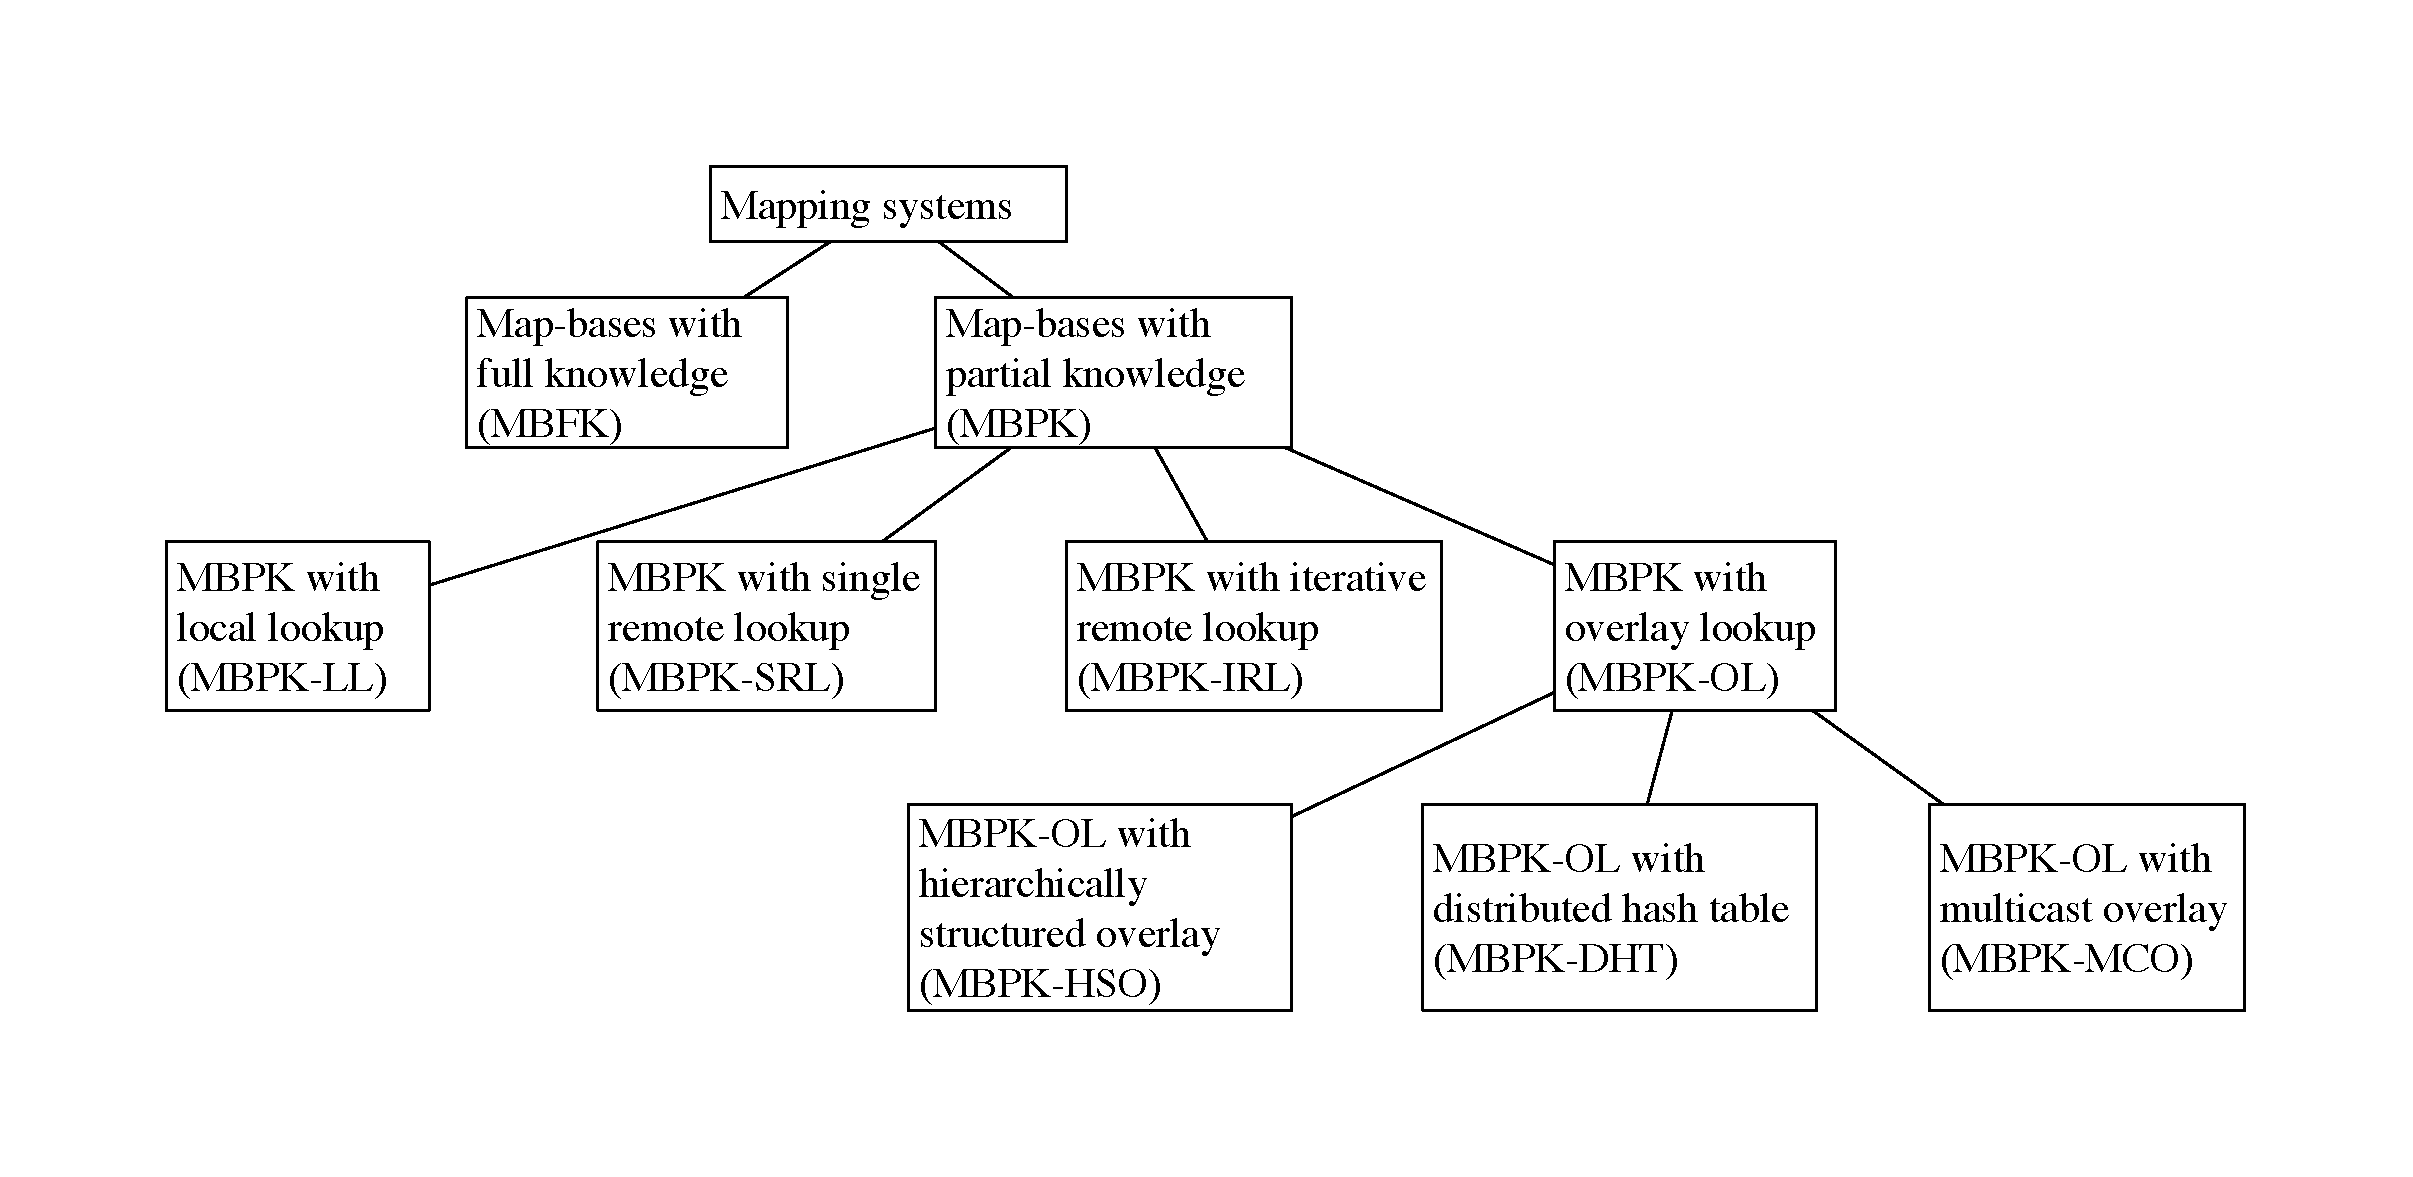
\includegraphics[width=\textwidth]{Pics/Hierarchical_taxonomy_of_mapping_systems.eps}
	\caption{Hierarchical taxonomy of mapping systems (from \cite{info3-articles-2013-06})}
	\label{Hierarchical_taxonomy_of_mapping_systems}
\end{figure}
%-< END FIGURE >--------------------------------------------------------------------
The current BGP-based Internet routing architecture relies on a push model, in which routing information is pushed to the whole Internet. The Locator/Identifier Split-based Internet routing instead relies on a pull model, where the \emph{\acrfull{mds}} provides a mapping upon an explicit query,\footnote{The terms \emph{\acrfull{mds}} and \emph{mapping system} are used interchangeably in this dissertation.}  where routing information is pulled only when actually needed. This paradigm shift requires making routing information available in an on-demand manner. % To achieve this purpose, a new system called \emph{Mapping System} is introduced.
Fig.~\ref{Hierarchical_taxonomy_of_mapping_systems} shows the current possible taxonomy of mapping systems~\cite{info3-articles-2013-06}. So far, several mapping systems have been proposed for LISP, such as: LISP-TREE~\cite{lispTree}, LISP-NERD (Not-so-novel EID to RLOC Database)~\cite{lear2013nerd} and LISP-CONS (Content distribution Overlay Network Service for LISP)~\cite{brim2008lisp}. However, only two have been deployed: \emph{LISP Alternative Logical Topology (LISP+ALT)}~\cite{rfc6836} and \emph{LISP Delegated Database Tree (LISP-DDT)}~\cite{lispDDT}.


\subsubsection{LISP+ALT}
\label{sec:lispalt}
%-< FIGURE >--------------------------------------------------------------------
\begin{figure}[!t]
	\centering
	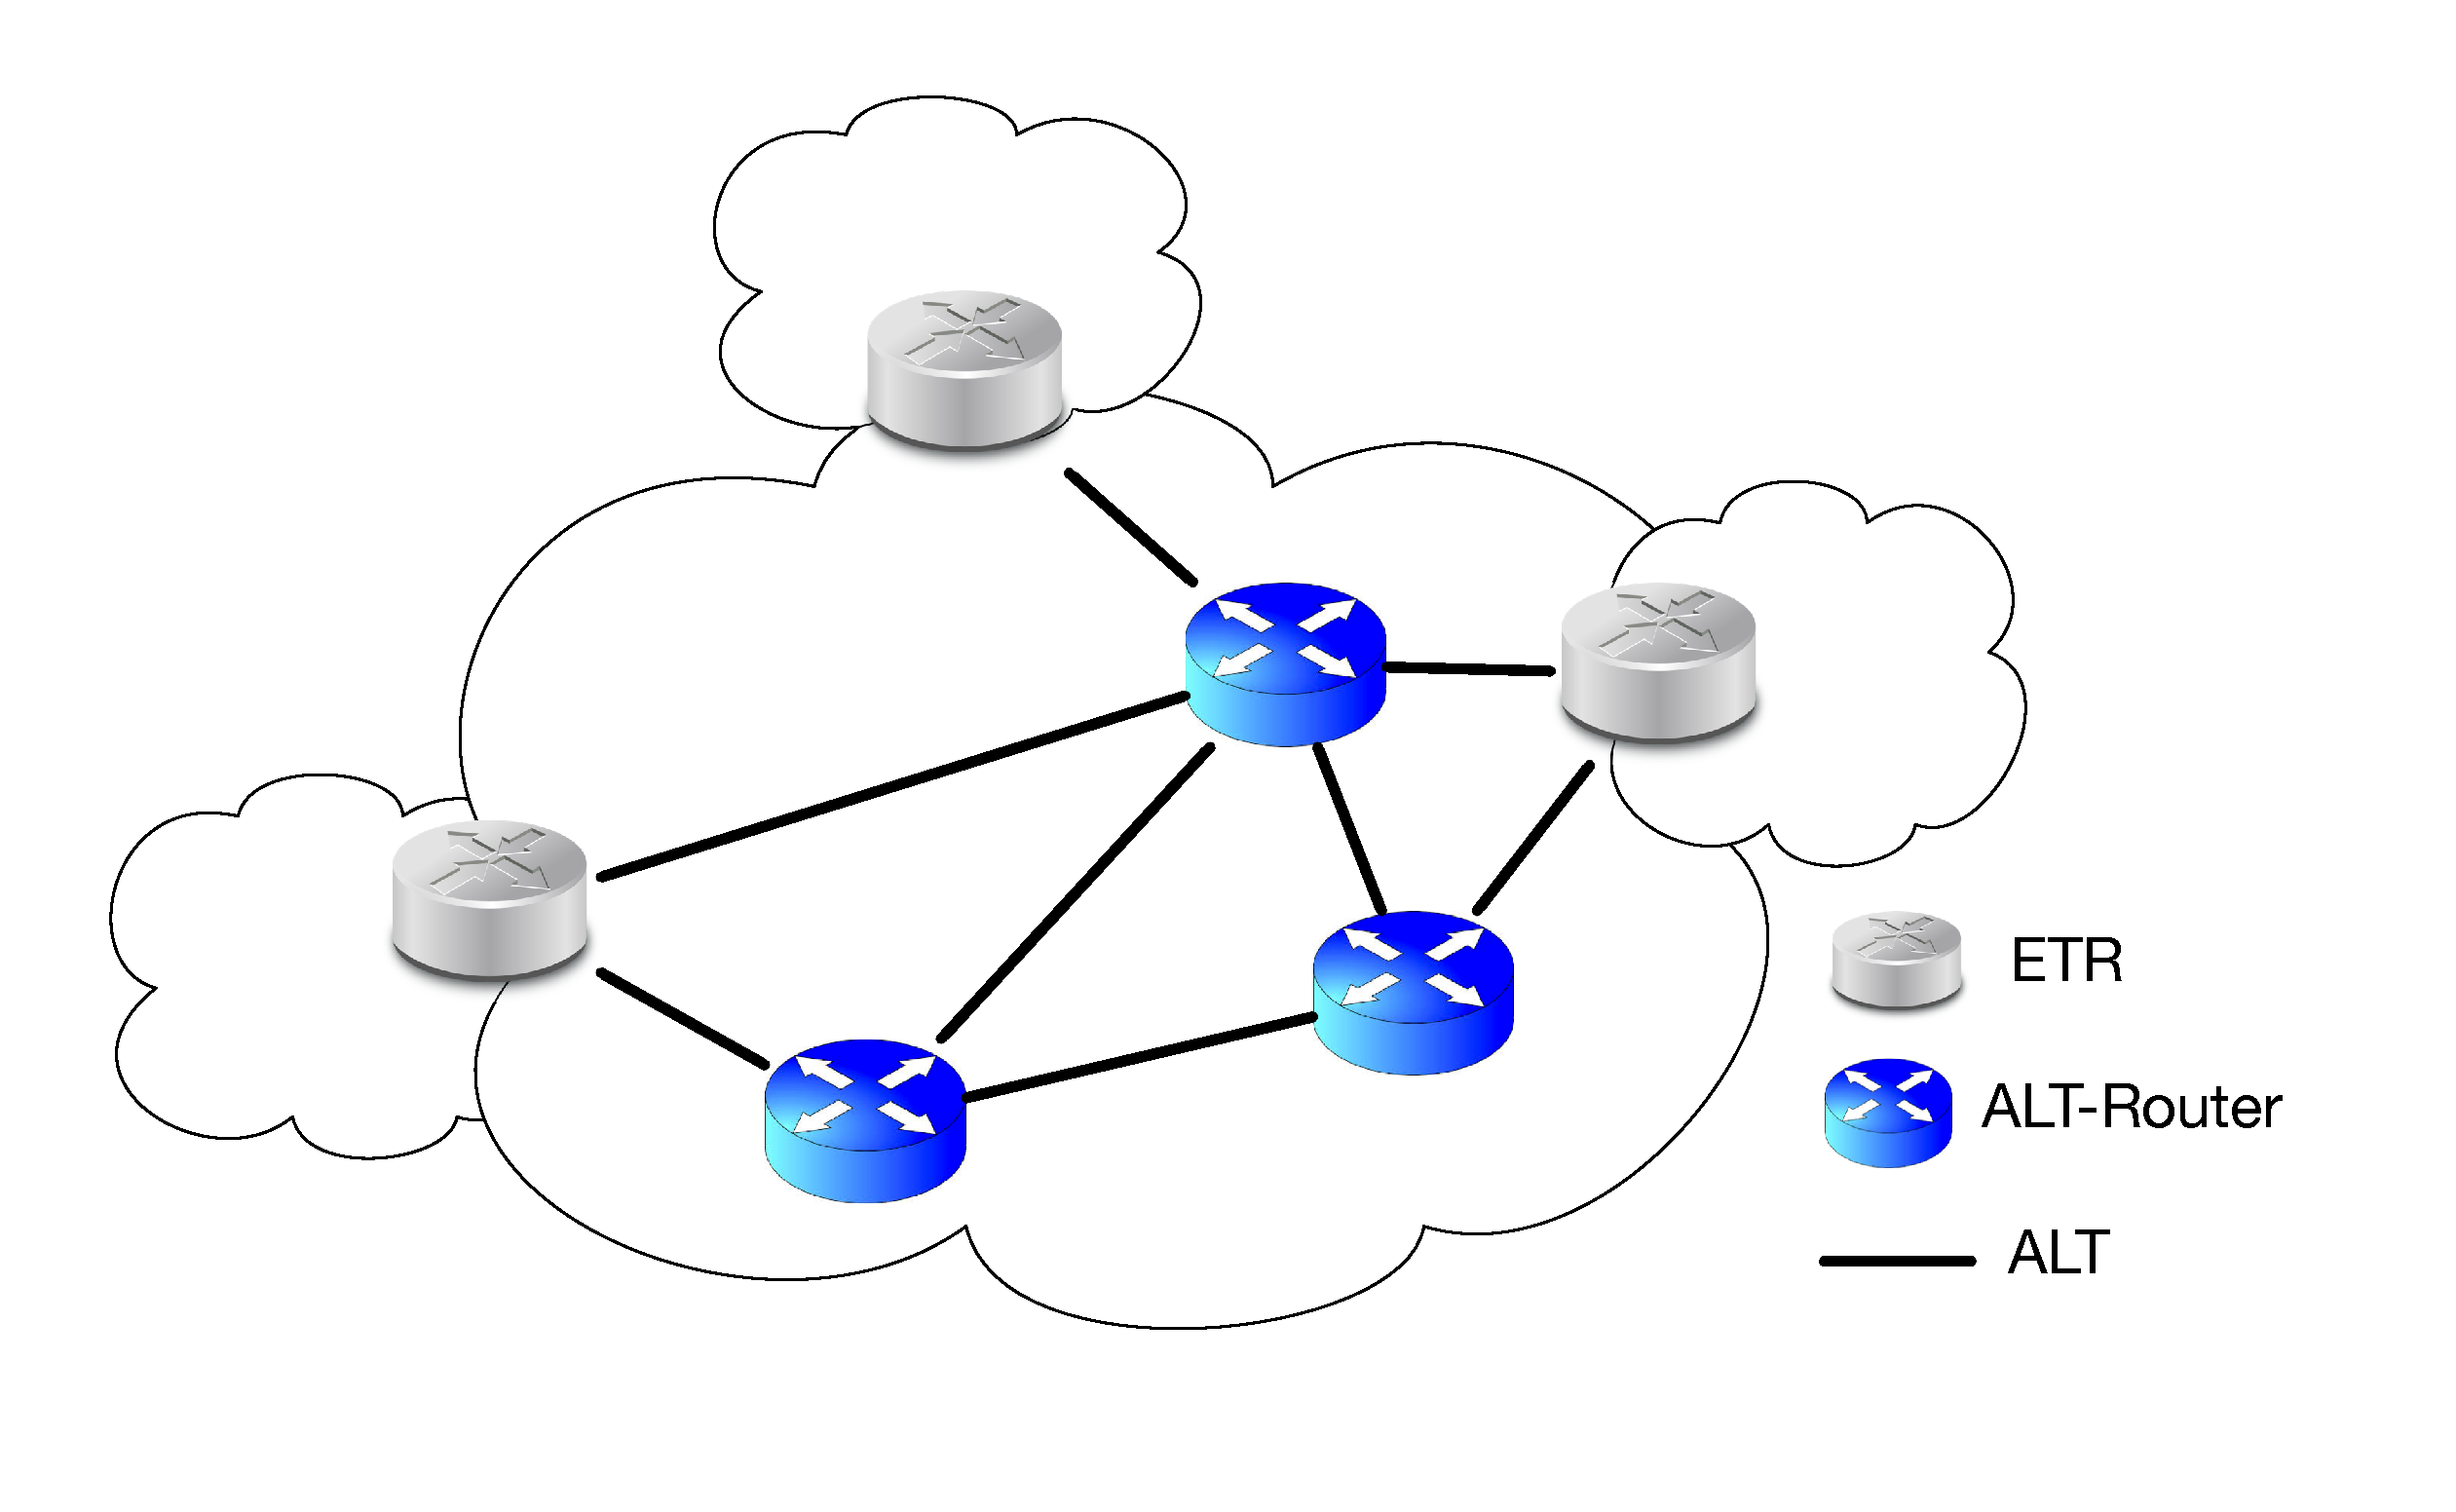
\includegraphics[width=0.9\textwidth]{Chapter2/Pics/LISP_ALT.eps}
	\caption{Illustration of the LISP+ALT topology}
	\label{LISP_ALT}
\end{figure}
%-< END FIGURE >--------------------------------------------------------------------
\emph{LISP+ALT} was the initial mapping system for LISP, where the \acrshort{etr}s store mappings they are authoritative for~\cite{lispCCR}. The basic idea is to use BGP to construct an overlay, named Alternative Logical Topology (ALT), to establish reachability between \acrshort{etr}s via tunnels (e.g., GRE tunnels~\cite{farinacci2000rfc}). As shown in Fig.~\ref{LISP_ALT}, the routers in the ALT are called ALT-Routers. Each ALT–Router maintains a BGP session with its neighbor and announces the EID–prefixes it is authoritative for. These EIDs are then routable in the ALT. Note that the ALT–Routers only exchange aggregated EID-prefixes that can be reached through them between neighbors, but they do not contain the mapping information. To get a mapping, an \acrshort{itr} constructs a Map-Request for the queried EID by using its own RLOC as source address and the queried EID as destination address, then sends it to an ALT-Router. The Map-Request is forwarded over the ALT and eventually reaches an originator \acrshort{etr} for the EID-prefix that matches the destination EID. This \acrshort{etr} resolves the Map-Request and directly sends back a Map-Reply to the inquirer \acrshort{itr}, this time not using the ALT. LISP-ALT belongs to the Map-Bases with Partial Knowledge using Hierarchically Structured Overlay (MBPK-HSO) in Fig.~\ref{Hierarchical_taxonomy_of_mapping_systems}.


\subsubsection{LISP-DDT}
\label{sec:lispddt}
%-< FIGURE >--------------------------------------------------------------------
\begin{figure}[!t]
	\centering
	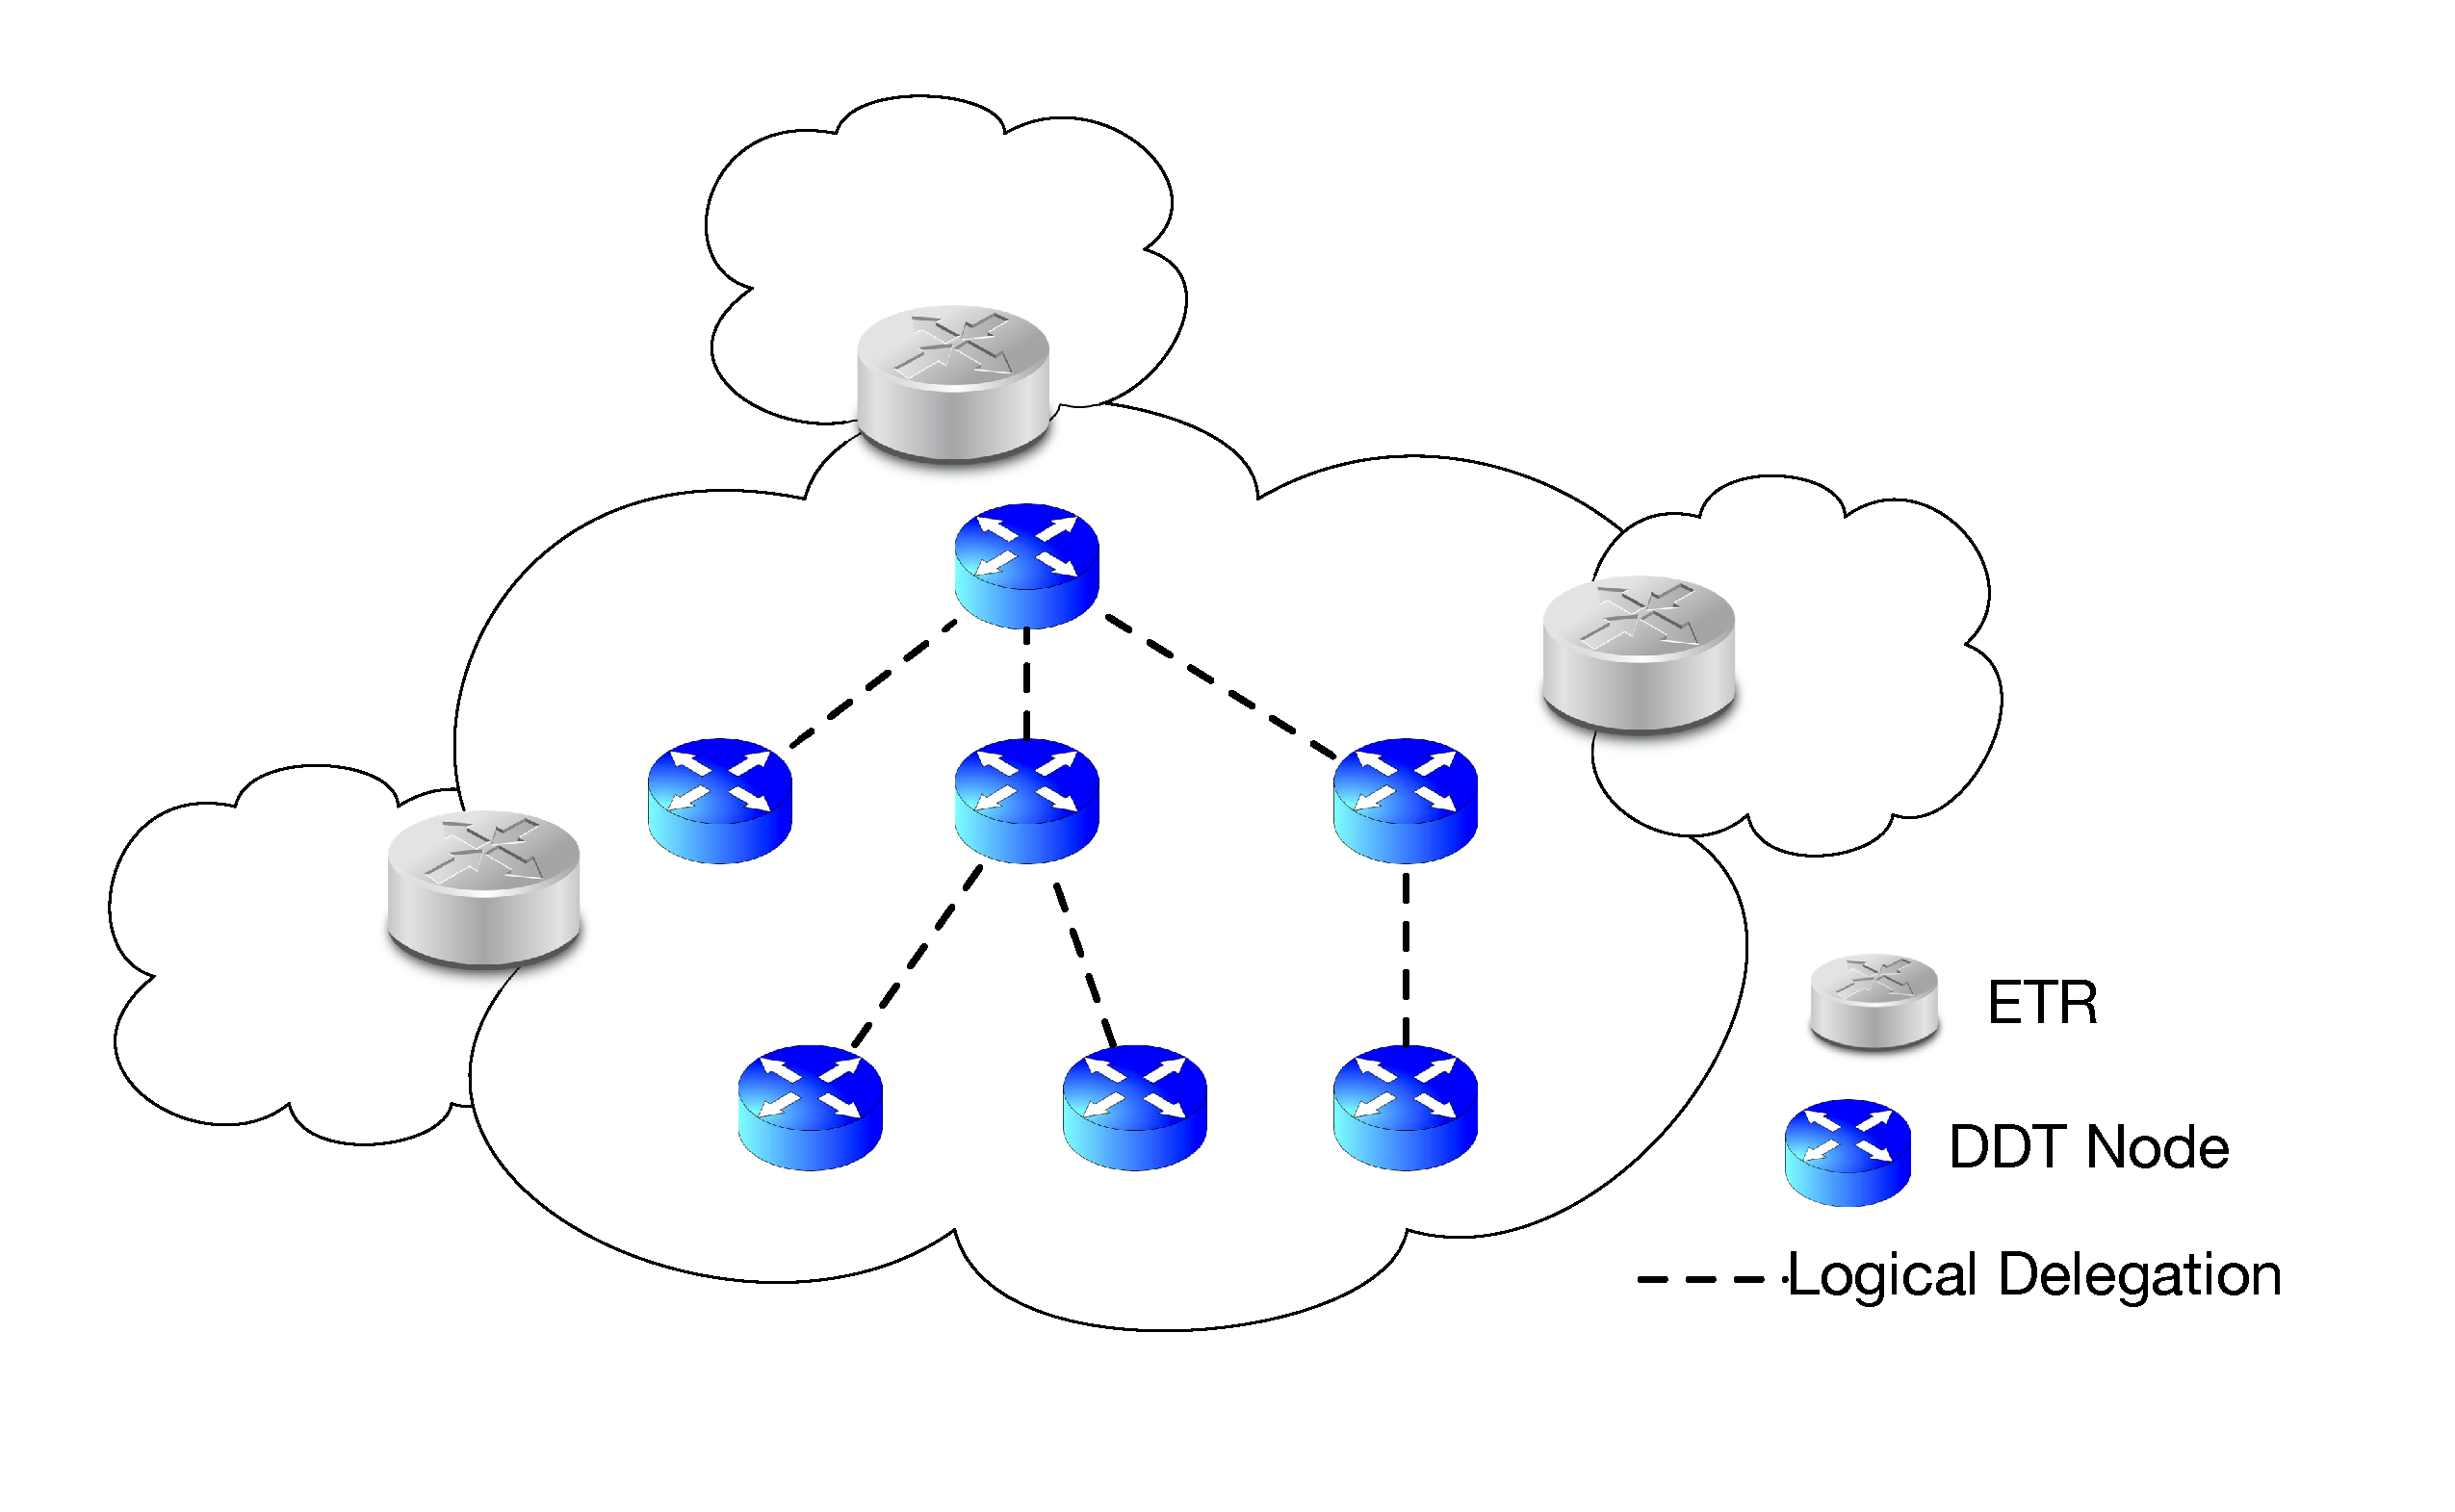
\includegraphics[width=0.9\textwidth]{Chapter2/Pics/LISP_DDT.eps}
	\caption{Illustration of the LISP-DDT topology}
	\label{LISP_DDT}
\end{figure}
%-< END FIGURE >--------------------------------------------------------------------
\emph{LISP-DDT} is a hierarchical distributed database that embodies the delegation of authority to provide mappings from LISP EIDs to RLOCs . Its hierarchical organization is shown in Fig.~\ref{LISP_DDT}. It consists of \emph{Map-Resolvers (MRs)} and \emph{Map-Servers (MSes)} to provide a simplified "front end". The MR is a network infrastructure component that accepts LISP Encapsulated Map-Requests from an \acrshort{itr} and resolves the mapping using a DNS-like distributed database. The MS learns of EID-Prefix mapping entries (a list of EID-Prefixes plus a set of RLOC tuples) from \acrshort{etr}s. The hierarchy is maintained as a tree where a root server is responsible for the entire EID space. This space is divided into several portions and each one is managed by one of the root’s children.
% where each node is responsible for a specific part of the EID-prefixes. A child node is responsible for a portion of the EID-prefixes of its parent. 
Mapping information is only stored at the tree leaves, which are made of MSes. Intermediate nodes only maintain pointers to their children.

If an \acrshort{itr} cannot find a mapping in its LISP Cache for a new flow, it sends a query, called \emph{Map-Request}, to a \acrshort{mr}~\cite{rfc6833}. The \acrshort{mr} determines whether the queried destination IP address is an EID. If not, a \emph{Negative Map-Reply} is directly returned; otherwise, the root server is queried. The root replies with a pointer to its child node responsible for the queried EID. The process is recursively repeated to find the child root of the sub-tree where a mapping can be retrieved for the queried EID. When the leaf is reached, the mapping is then retrieved by sending a Map-Request to the \acrshort{etr} authoritative for the matching EID-prefix. The \acrshort{etr} in turn directly replies a \emph{Map-Reply} message containing the whole requested mapping information to the \acrshort{itr} initiating the query.

When an \acrshort{etr} first contacts an \acrshort{ms} after restarting or changing its database, it sends the Map-Register messages to the \acrshort{ms} to publish its EID-prefixes as well as the mapping information. % at an increased frequency, up to one every 20 seconds. 
For maintaining the association, the registration interval should be expanded to at least 1 minute. If the MS has not received a valid Map-Register within the past 3 minutes, it removes the registration of this \acrshort{etr}. If the "want-map-notify" (M-bit) flag is set in Map-Register, the received MS needs to send back a Map-Notify message to inform the \acrshort{etr} that the Map-Register has been received and processed. If the "proxy Map-Reply" flag (P-bit) is set, the MS answers the Map-Requests to the queried \acrshort{itr} by providing the mapping information on behalf of the \acrshort{etr}. \acrshort{mr}s offer an interface to the \acrshort{mds} for the \acrshort{xtr}s, so that the whole complex \acrshort{mds} mechanism can be hided.


\subsection{Communication between two LISP-sites}
\label{sec:communication_2_lisp}
%-< FIGURE >--------------------------------------------------------------------
\begin{figure}[!t]
	\centering
	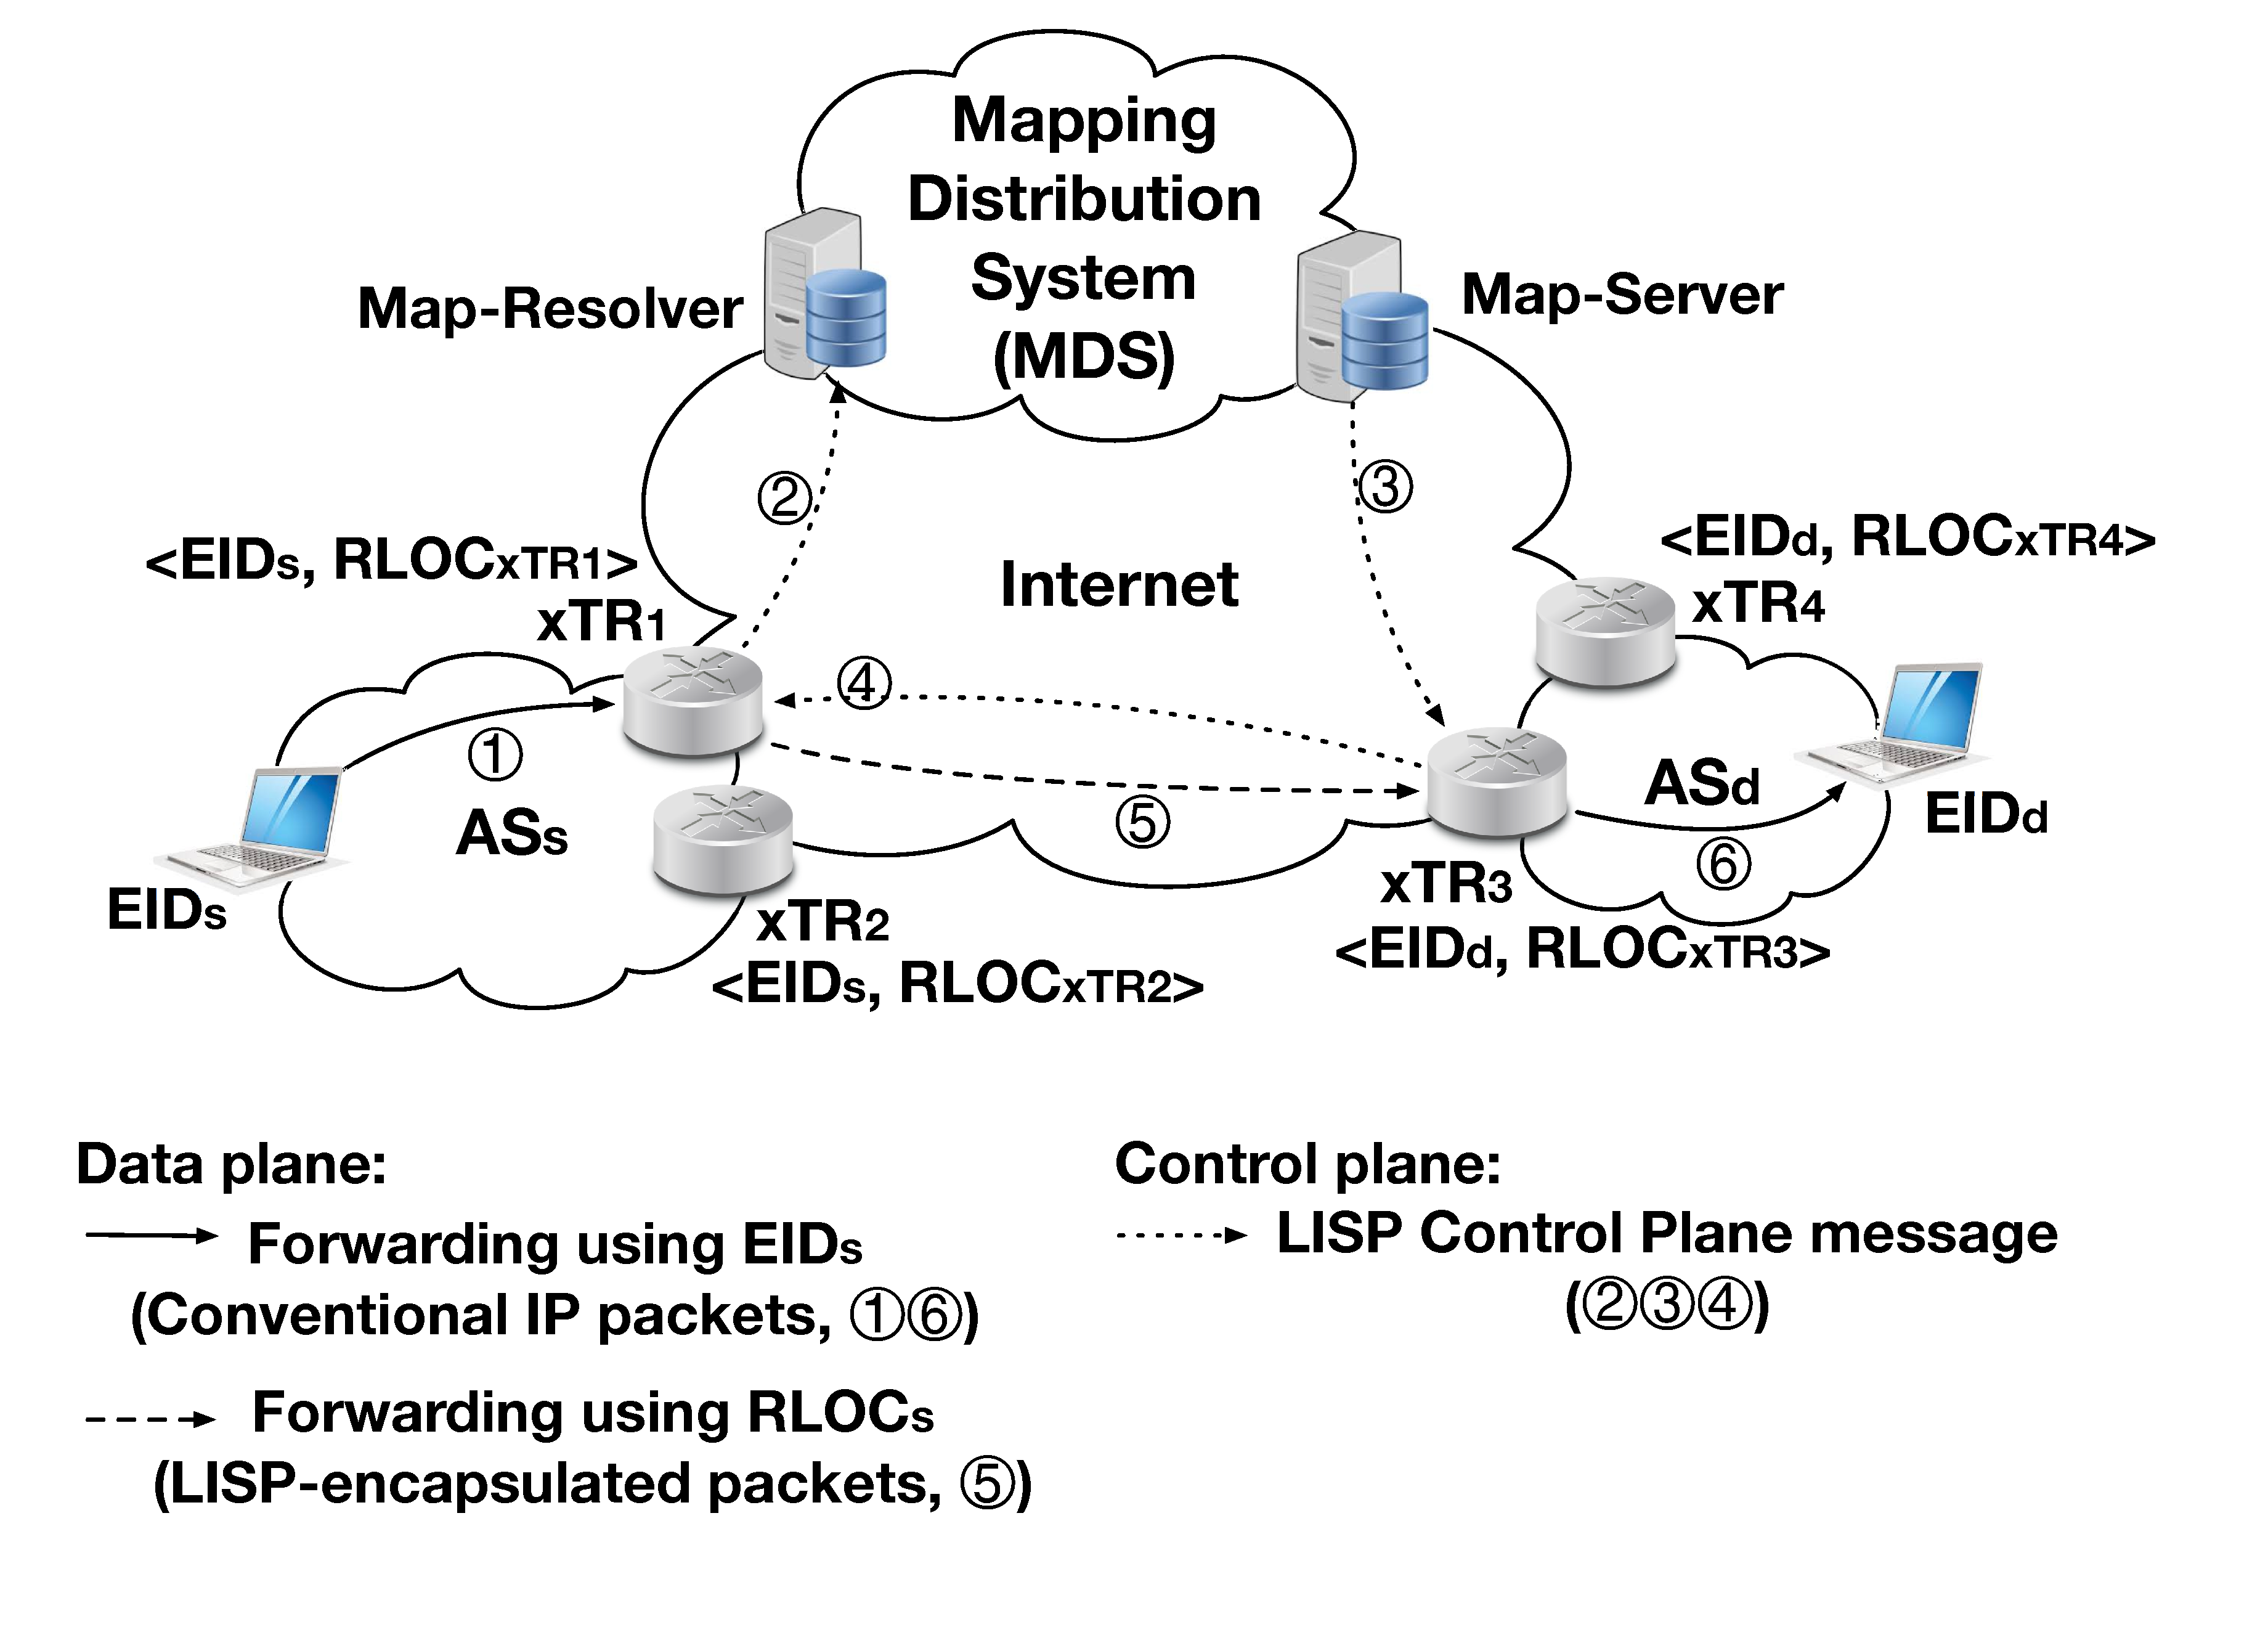
\includegraphics[width=0.9\textwidth]{Pics/LISP_D_C_planes.eps}
	\caption{LISP architecture overview}
	\label{LISP_archi}
\end{figure}
%-< END FIGURE >--------------------------------------------------------------------
We use Fig.~\ref{LISP_archi} as an example to describe how the LISP packets are processed in details in the case of the packets exchange between two LISP-sites.

When the host in the $AS_s$ communicates with the host in the $AS_d$, it uses $EID_s$ as source address and $EID_d$ as destination address. After the conventional IP routing to $xTR_1$ (the function of \acrshort{itr} and \acrshort{etr} are combined together in Fig.~\ref{LISP_archi}) labeled as \emph{"1"}, $ITR_1$ first checks in its mapping cache~\cite{lispCacheCost} to find out the association between $EID_d$ and its RLOC. If there is no record, it sends a Map-Request to Map-Resolver (MR), labeled as \emph{"2"}. \acrshort{mr} searches which \acrfull{ms} stores the mapping information of $EID_d$ and forwards the Map-Request to that \acrshort{ms}. If \acrshort{ms} is authoritative (i.e., acts as a proxy), it directly returns back a Map-Reply containing the mapping information (this procedure is not labeled in the figure). If not, after forwarding the Map-Request within \acrshort{mds} with the procedure described in Sec.~\ref{sec:lispddt} to \acrshort{ms} and then to the destination side (label \emph{"3"}), $xTR_1$ receives a Map-Reply from one of \acrshort{etr}s of $EID_d$ (label \emph{"4"}). If the Map-Reply shows that the priority of $ETR_3$ is higher than $ETR_4$, then the $ITR_1$ encapsulates the packets by adding $RLOC_{ETR_3}$ as the destination address and $RLOC_{ITR_1}$ as the source address in the outer header and sends the encapsulated packets through the Internet as labeled \emph{"5"} in Fig.~\ref{LISP_archi}. Once $ETR_3$ receives these packets, it decapsulates and forwards them by using the original IP packets (label \emph{"6"}). If the destination site is not a LISP-site, the MR directly returns back the Map-Reply without mapping information to $ITR_1$.

Based on LISP architecture, there are three types of outcomes for a query:
\begin{itemize}[noitemsep,topsep=0pt]
%\begin{inparaenum}[(i)]
	\item \emph{LISP Map-Reply}, means that the queried IP address belongs to a LISP site (i.e., EID) and the Map-Reply contains the mapping information for this site, including: the association between the EID-prefix that queried EID belongs to, and the list of RLOC tuples $<$RLOC, Priority, Weight$>$ of the destination site.
	\item \emph{Negative Map-Reply}, means that the prefix covering the queried IP address belongs to a non-LISP site (i.e., conventional site), and the Map-Reply contains no mapping information. We consider these two kinds of replies as successful queries.
    \item \emph{No Map-Reply}, means that the \acrshort{xtr} does not receive any reply during a certain time. According to the standard described in~\cite{rfc6830}, the time-out is set to 3 seconds. But this value can be modified in the implementation to adapt the experiment needs. In this case, we consider the query as failed.
%\end{inparaenum}
\end{itemize}


%-< SECTION >--------------------------------------------------------------------
\section{Interworking With Legency Internet}
\label{sec:background_Interworking}
% \begin{itemize}[noitemsep,topsep=0pt]
%     \item Describe what is PxTR.
%     \item How it works when a terminal behind LISP-site communicates with a terminal on the legacy Internet.
% \end{itemize}

Sec.~\ref{sec:communication_2_lisp} describes how the LISP packets are exchanged between two LISP-sites. This section discusses how the packets are processed when a terminal behind LISP-site communicates with a terminal on the legacy Internet.

%-< FIGURE >--------------------------------------------------------------------
\begin{figure}[!t]
	\centering
	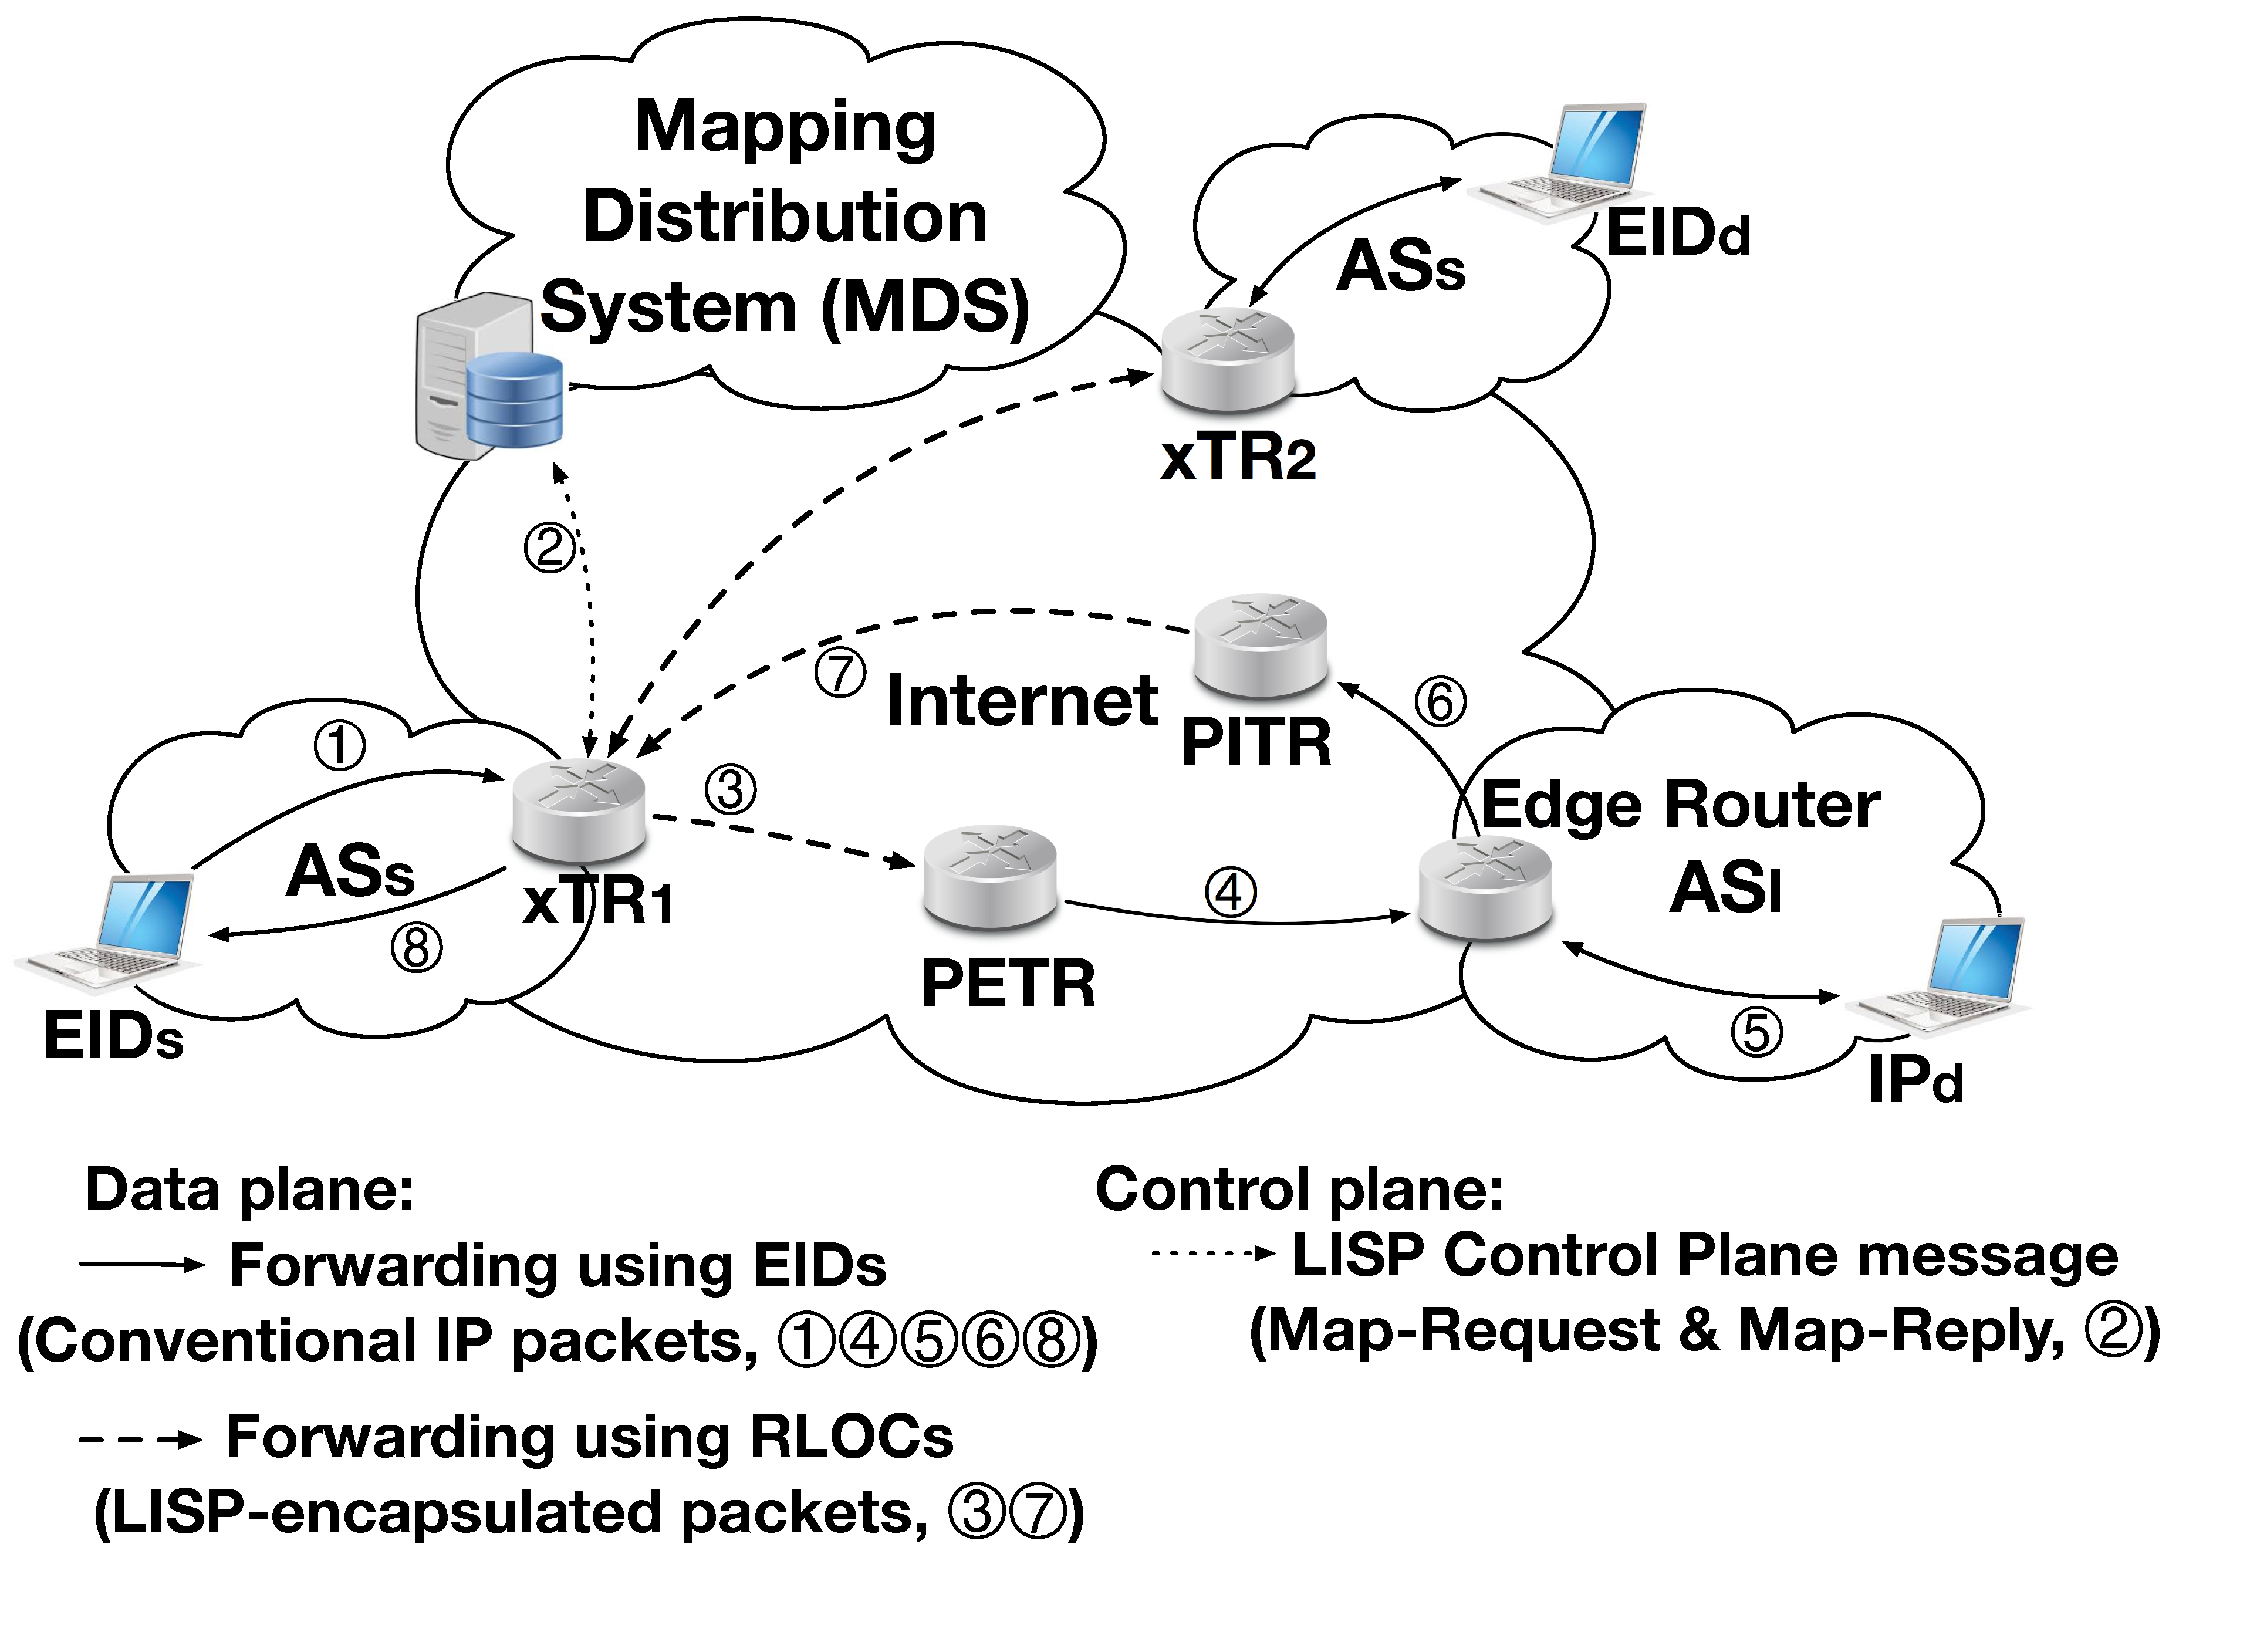
\includegraphics[width=0.9\textwidth]{Pics/LISP_archi_PxTR.eps}
	\caption{LISP architecture with the packets forwarding sequence}
	\label{LISP_archi_PxTR}
\end{figure}
%-< END FIGURE >--------------------------------------------------------------------
Although EIDs are syntactically identical to IPv4 or IPv6 addresses, routes to them are not announced in the global routing system, so an interoperability mechanism is needed for non-LISP-speaking sites to exchange traffic with LISP-speaking sites. Thus, two new network elements are introduced: LISP \acrfull{pitr} and LISP \acrfull{petr}. The \acrshort{pitr} acts as an intermediate LISP \acrshort{itr} for the hosts on legacy Internet. It is in charge of announcing one or more highly aggregated EID-Prefixes on behalf of LISP-sites into the public Internet and receives the traffic from the public Internet to encapsulate them as LISP packets. The \acrshort{petr} acts as an \acrshort{etr} for traffic destined to non-LISP sites. It receives the traffic from the \acrshort{itr}s, decapsulates the LISP packets into conventional IP packets and sends them to the legacy Internet.

Fig.~\ref{LISP_archi_PxTR} shows an example for the packets exchanging between LISP-site and non LISP-site (i.e., legacy Internet). The host with $EID_s$ in the $AS_s$ exchanges the packets with the host with the $IP_d$ in the $AS_l$. With the same procedure introduced in Sec.~\ref{sec:communication_2_lisp} labeled as \emph{"1"} and \emph{"2"} in Fig.~\ref{LISP_archi}, the original IP packets are sent from host to $xTR_1$, and the later one sends the Map-Request to \acrshort{mds} to query the mapping information. Since the destination is in a non-LISP-Site, the MR directly returns back the Map-Reply without mapping information (i.e., Negative Map-Reply) to $xTR_1$, the packet can either be sent non-encapsulated or the $xTR_1$ encapsulates it using the statically configured RLOC of the \acrshort{petr} as the outer destination address and forwards the LISP packets there. When \acrshort{petr} receives the LISP-encapsulated packets, it performs a decapsulation as an \acrshort{etr} and then forwards the inner IP packets to the legacy destination host by using the normal BGP routing, labeled as procedure \emph{"4"} and \emph{"5"} in Fig.~\ref{LISP_archi_PxTR}. 

When the packets come back, they are forwarded in a traditional way from the host with address $IP_d$ in $AS_l$ to the \acrshort{pitr}, denoted as procedure \emph{"5"} and \emph{"6"} in Fig.~\ref{LISP_archi_PxTR}. A \acrshort{pitr} shares many characteristics with \acrshort{itr}s, as it also queries the mapping information of destination to the \acrshort{mds} and encapsulates the non-LISP Internet traffic into LISP-encapsulated packets and route them to their destination RLOCs (label \emph{"7"}). Target $ETR_1$ then dencapsulates the packets and send them to the destination host $EID_s$. The \acrshort{petr} and \acrshort{pitr} can be noted together as \acrshort{pxtr} if they are located on a same physical router.



%-< SECTION >--------------------------------------------------------------------
\section{Mapping Cache Update Mechanisms}
\label{sec:updateMechanisms}
% When the \acrshort{etr}s change their mappings, the only way that remote \acrshort{itr} can get the updated mapping information is to re-request the mapping. Thus, two protocol approaches are proposed to get the latest mapping. They are Solicit-Map-Request and Map-Versioning.
Given that LISP mapping distribution is based on a pull model, in case that mapping changes occur in \acrshort{etr}s, the only way that makes remote \acrshort{itr}s be aware of such change and update the corresponding mapping information is to request again the mappings to \acrshort{etr}s. Thus, two mechanisms are proposed to notify \acrshort{itr}s that mapping has changed and they need to get the latest mapping: Solicit-Map-Request and Map-Versionning.


%-< SUB SECTION >--------------------------------------------------------------------
\subsection{Solicit-Map-Request (SMR)}
\label{sec:SMR}
Soliciting a Map-Request is used by \acrshort{etr}s to tell remote \acrshort{itr}s to update the mappings they have cached. When the mappings in the Database of an \acrshort{etr} changes, the \acrshort{etr} sends the Map-Requests with the \acrshort{smr} bit set (called \acrfull{smr} message) for each RLOC in its Cache. A remote \acrshort{itr} that receives the \acrshort{smr} message will take a check in its Cache whether the source RLOC of the \acrshort{smr} message, i.e., the RLOC of \acrshort{etr} with mappings change is in its Cache. If yes, the remote \acrshort{itr} sends a Map-Request to the MR (as shown in the left hand part of Fig.~\ref{SMR_schema}) or directly to the sender of \acrshort{smr} (as shown in the right hand part of Fig.~\ref{SMR_schema}). % In the case that the sender of \acrshort{smr} has the unique RLOC in the Locator-set of \acrshort{etr} that \acrshort{itr} caches, the \acrshort{itr} can only send the Map-Request to the MR, to avoid the \acrshort{etr} changes its RLOC and can not receive the SMR-invoked Map-Request any more. 
If the RLOC\yue{check} of sender is not in the Cache of \acrshort{itr} any longer, the later drops the \acrshort{smr} and does not send the Map-Request. The later situation occurs when the \acrshort{etr} sends the \acrshort{smr} to all RLOCs stored in its Cache, but the remote \acrshort{itr} actually has not sent the packets to it for a long time. Between sending the \acrshort{smr} message and receiving the new Map-Reply, the \acrshort{itr} continues to use the mapping information previously cached, and that may cause packet loss.
%-< FIGURE >--------------------------------------------------------------------
\begin{figure}[!t]
	\centering
	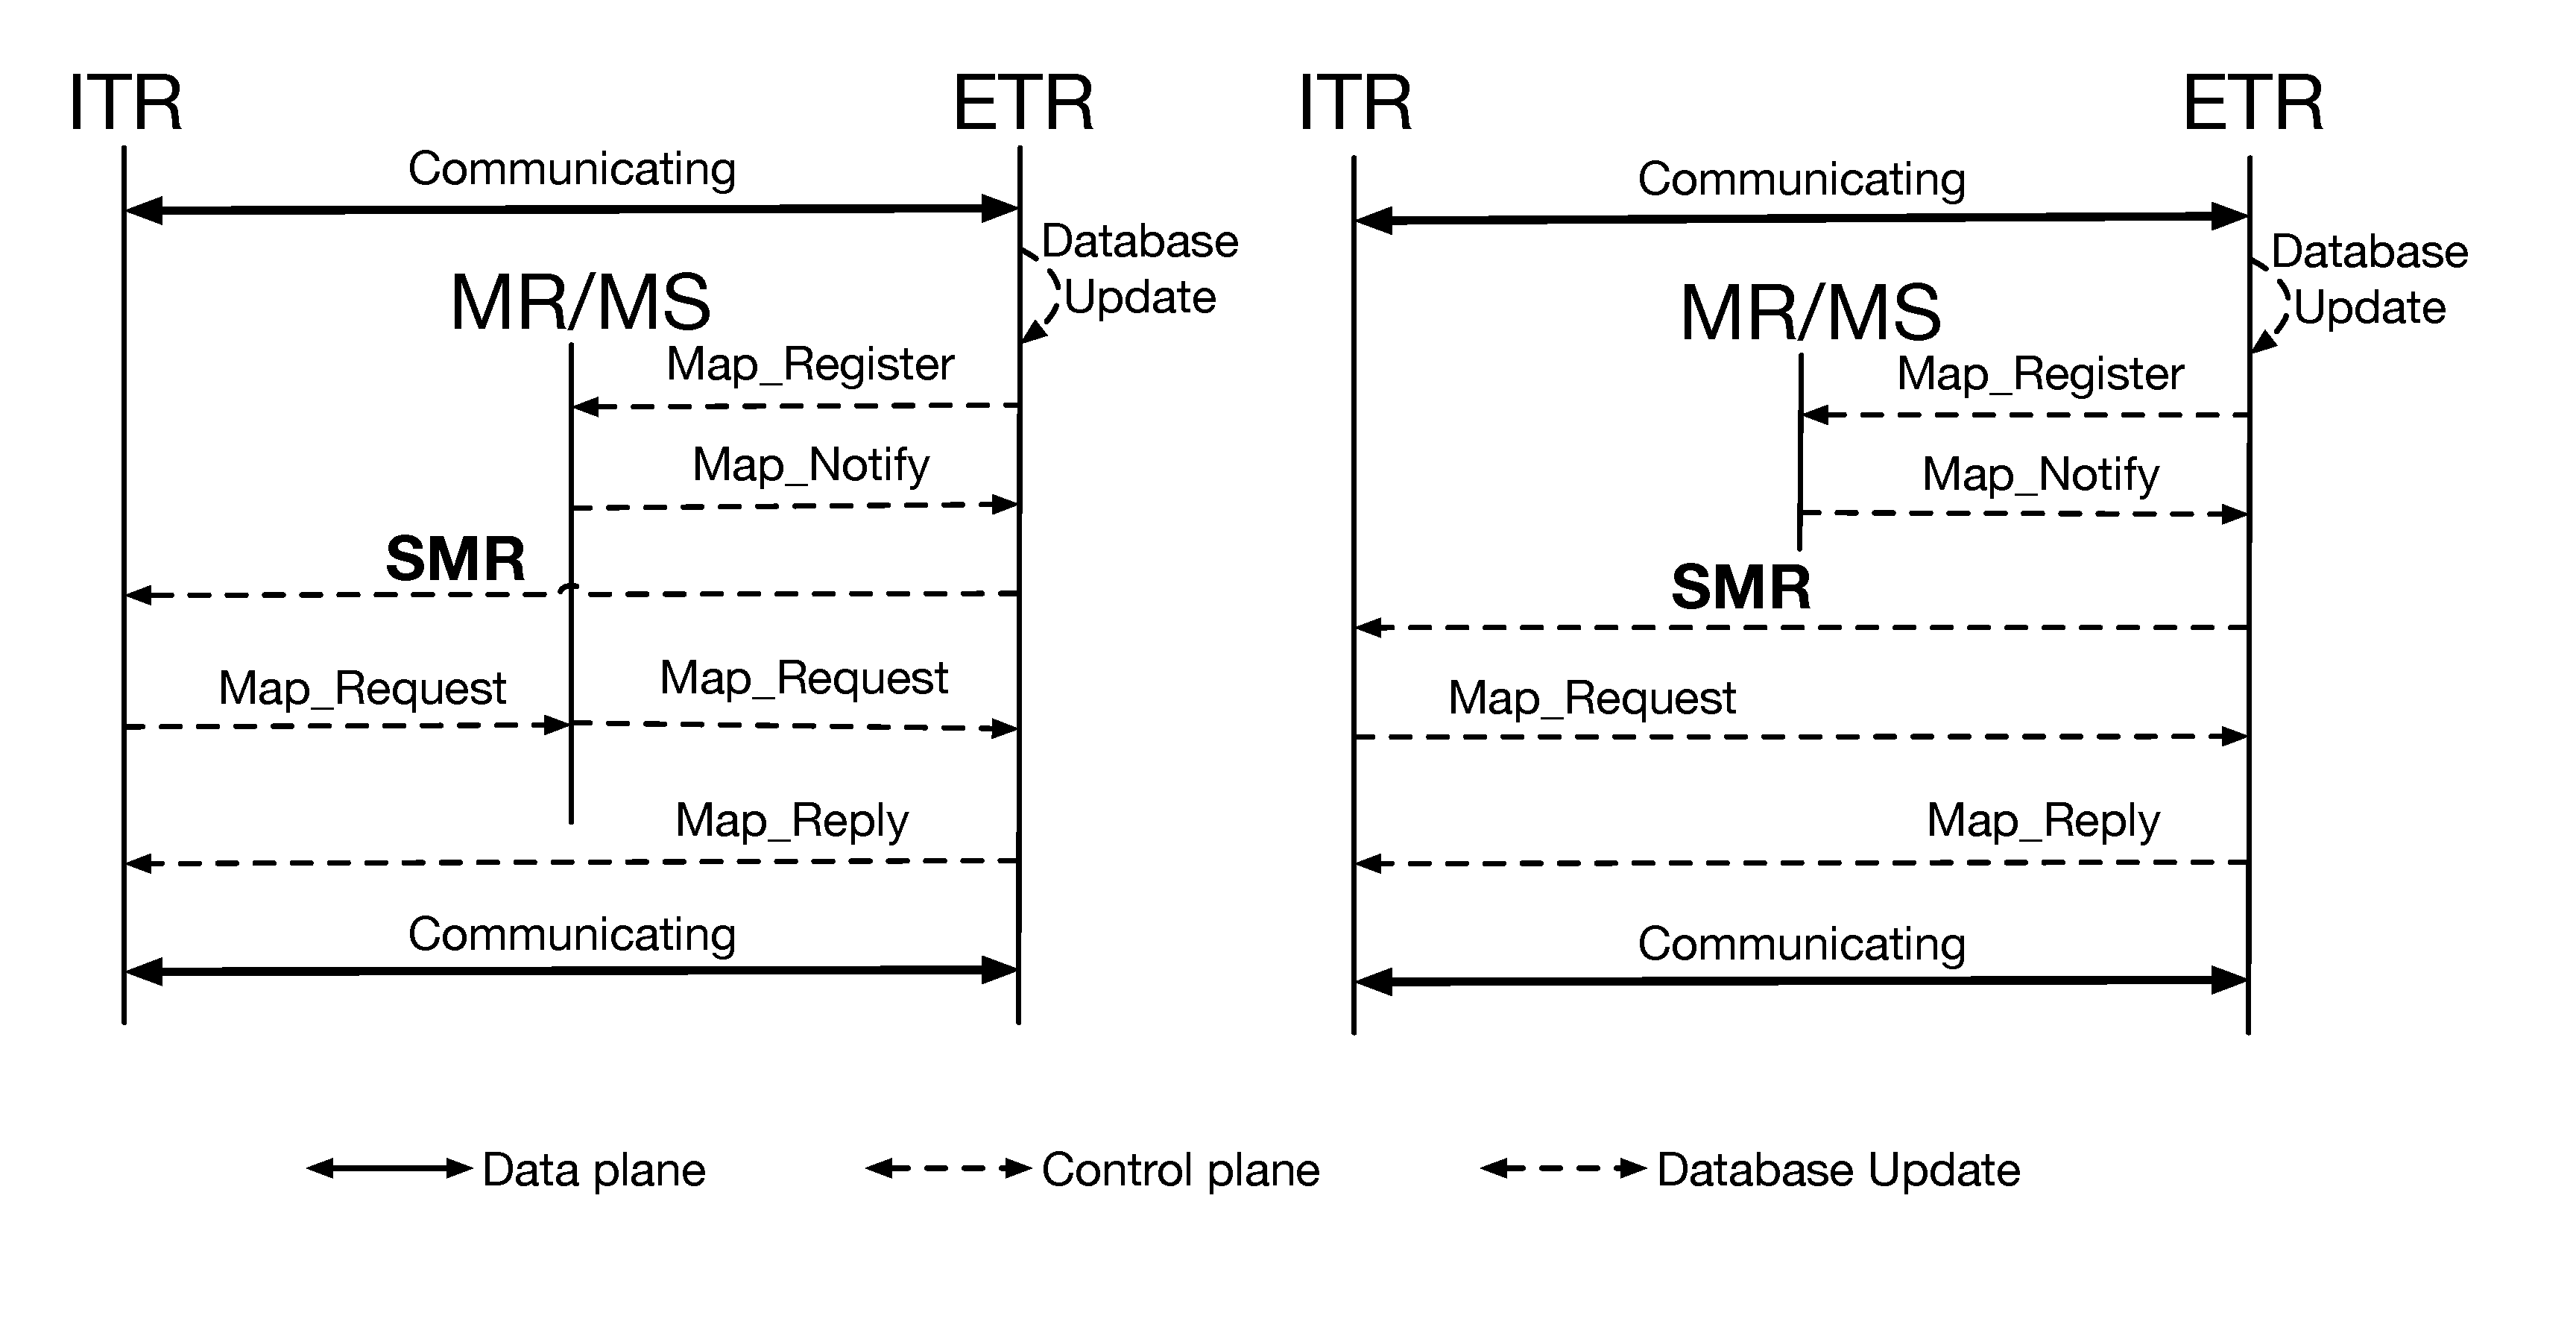
\includegraphics[width=\textwidth]{Pics/SMR_schema.eps}
	\caption{Packet sequence of LISP SMR mechanism}
	\label{SMR_schema}
\end{figure}
%-< END FIGURE >--------------------------------------------------------------------


%-< SUB SECTION >--------------------------------------------------------------------
\subsection{Map-Versioning}
\label{sec:MapVersionning}
%-< FIGURE >--------------------------------------------------------------------
\begin{figure}[!t]
	\centering
	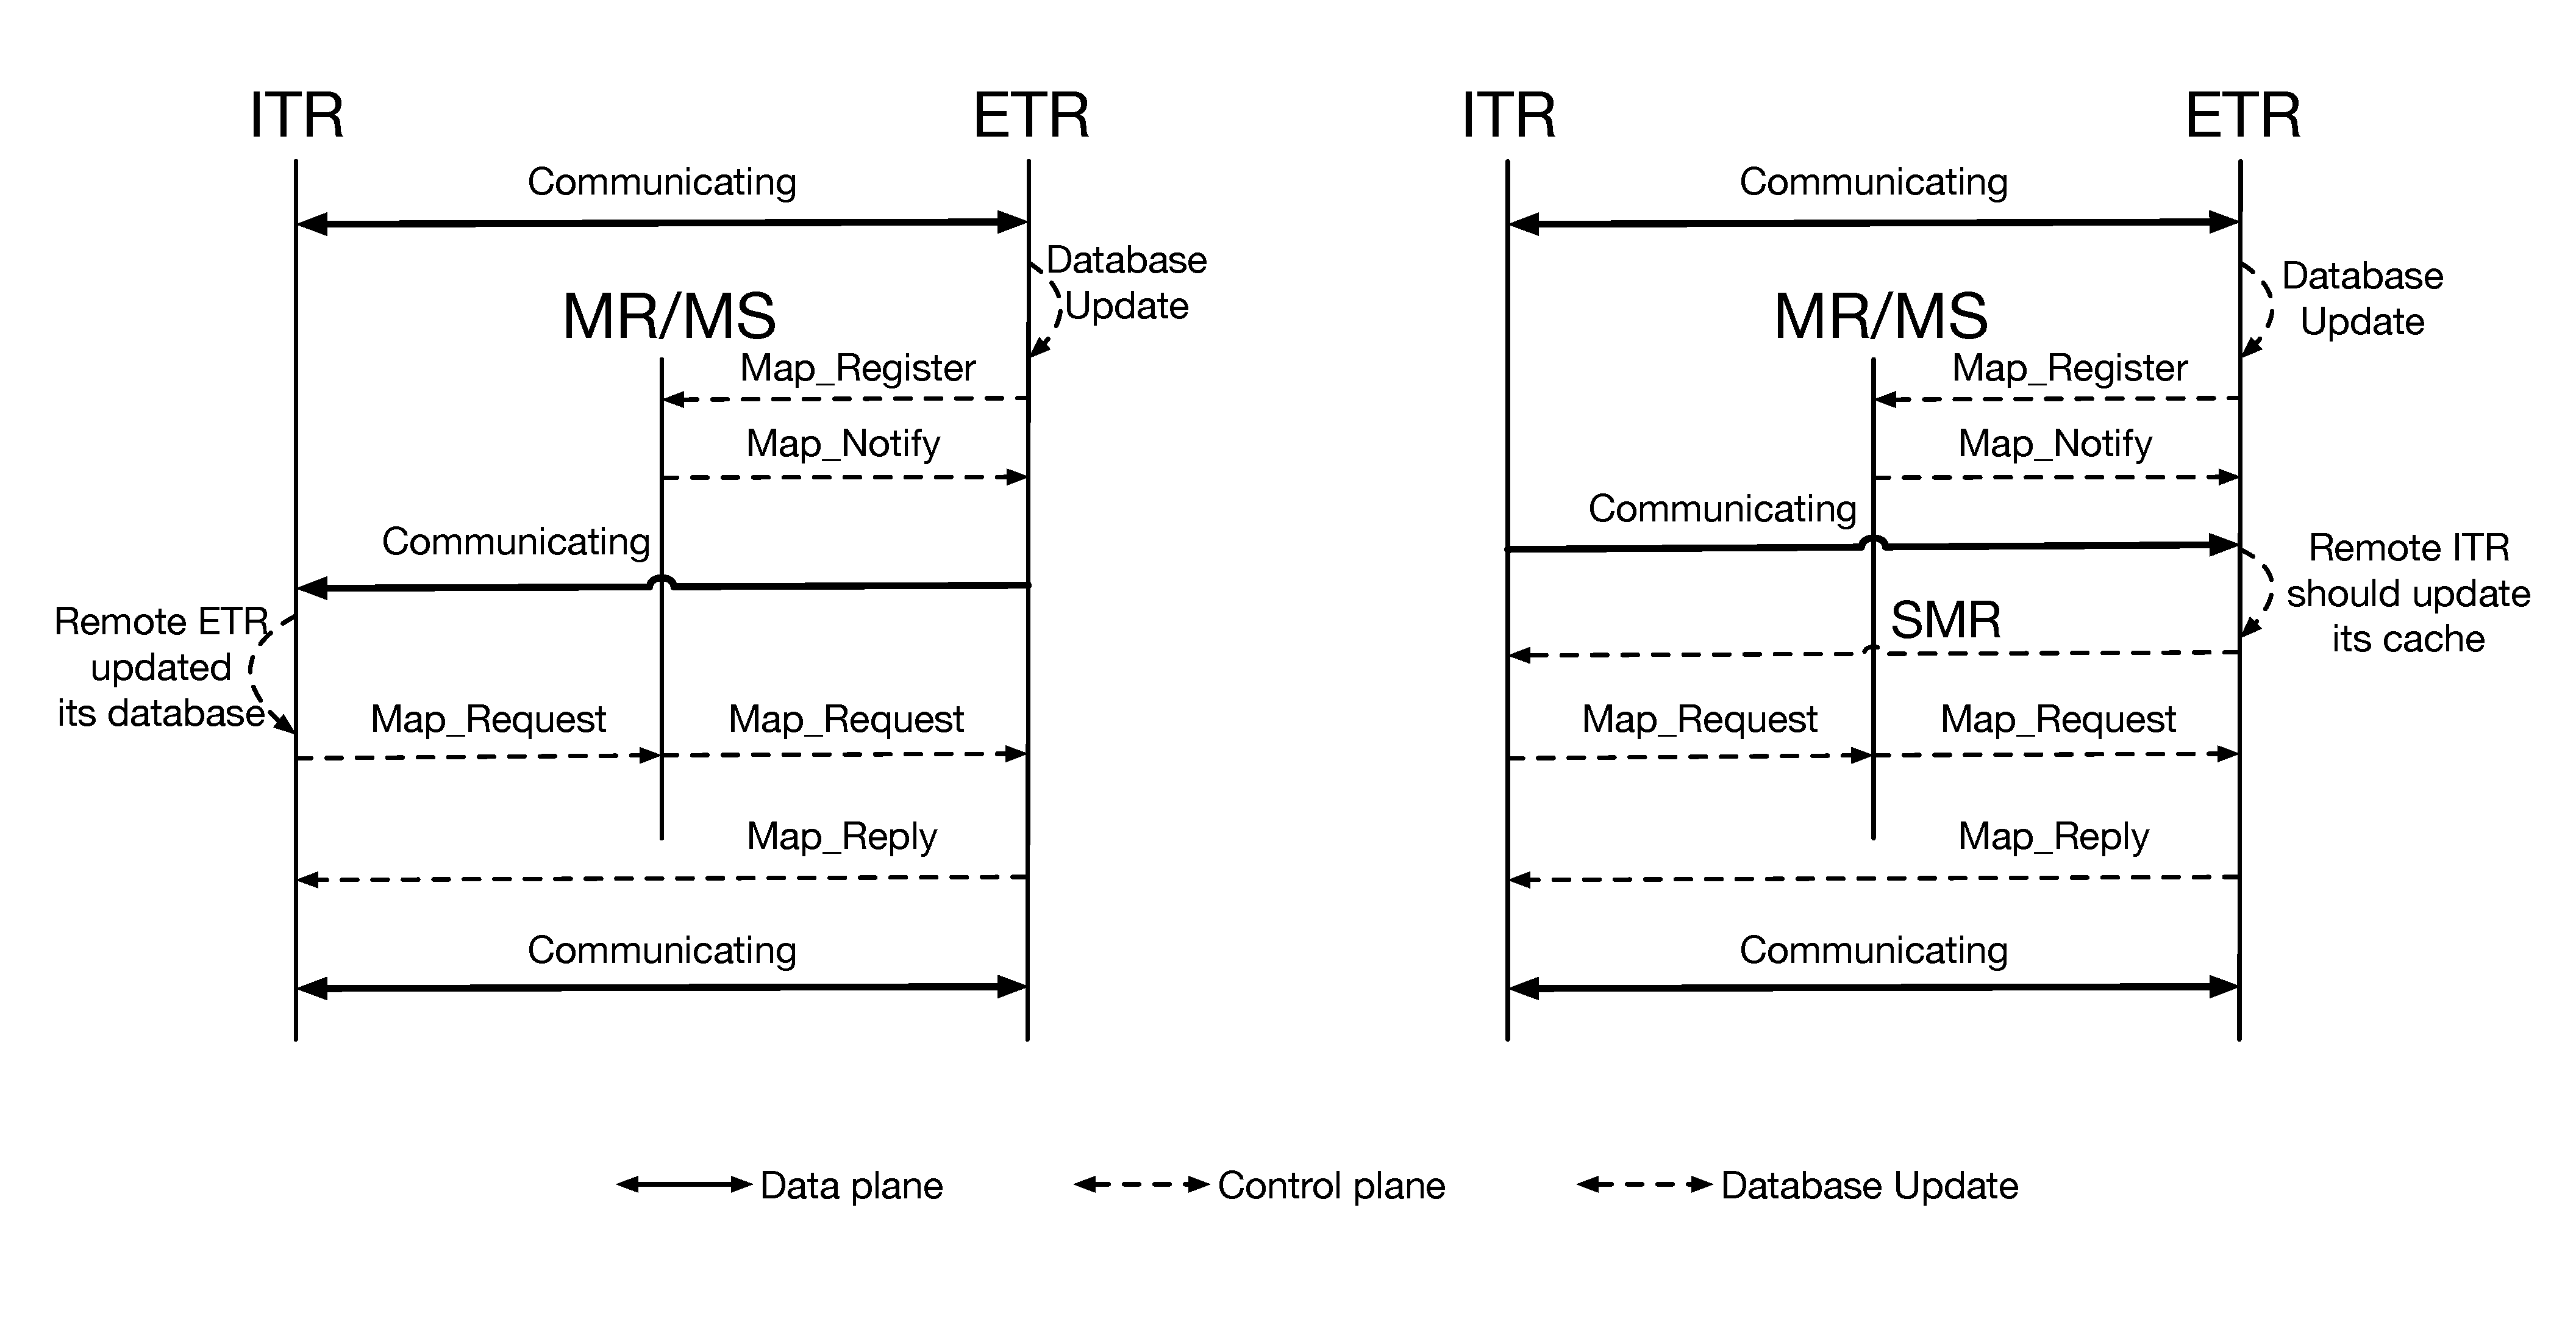
\includegraphics[width=\textwidth]{Pics/Map_versioning_schema.eps}
	\caption{Packet sequence of LISP Map-Versioning mechanism}
	\label{Map_versioning_schema}
\end{figure}
%-< END FIGURE >--------------------------------------------------------------------
Map-Versioning is used to inform through the Data Plane the \acrshort{xtr} that the mappings of a remote site changed and update the mapping information with the help of \acrshort{smr} message. Map-Versioning associates a Map-Version number to each LISP mapping information and transports such a version number in the LISP-specific header~\cite{rfc6834}. When a mapping changes, a new version number, normally incrementally higher than the previous one, is assigned to the updated mapping. When an \acrshort{itr} encapsulates a packet, it selects the version number assigned to the mapping stored in the Database as \emph{source RLOC version number}, and selects the version number assigned to the mapping contained in the Cache as \emph{destination RLOC version number}. When an \acrshort{etr} receives such packets and dencapsulates them, it makes a comparison between the received version number and the local one. If the source map version is higher than the one that \acrshort{etr} stores in its Cache, i.e., the mappings of remote \acrshort{itr} changed, the \acrshort{etr} sends a Map-Request to the MR or directly to the remote \acrshort{itr} to retrieve the latest mapping information (the left figure of Fig.~\ref{Map_versioning_schema}). If the destination map version is lower than the one contained in the Database of \acrshort{etr}, i.e., the local mappings changed but the remote site does not know, then the \acrshort{etr} sends a SMR to the remote \acrshort{itr} to let it update the cached mapping (the right figure of Fig.~\ref{Map_versioning_schema}).


%-< SECTION >--------------------------------------------------------------------
\section{LISP Mobility}
\label{sec:lisp_mobility}
%%-< SUBSUB SECTION >--------------------------------------------------------------------
%\subsection{Mobility at client-side}
%\label{subsubsec:mobility_user}
Nowadays, the explosion of mobile devices that need the massive mobile Internet traffic requires the evolution of mobile network architecture. Keeping the communication during the roaming without any interruption becomes a key point. Thanks to LISP separating the identifier of a host and the locator of the attachment point, the connection between two hosts can be kept alive while roaming. Because the EID, which is used as the inner address, is permanent, whereas only RLOC (used as the outer address) is changed. 

By using LISP mobility, it is possible 
\begin{inparaenum}[1)]
	\item to allow TCP connections to stay alive while roaming;
	\item to provide the shortest bidirectional data paths between a \acrfull{mn} and \acrfull{cn};
	\item to allow \acrshort{mn} to communicate with another \acrshort{mn} when both are roaming;
	\item not require fine-grained routes in the core network, nor the home-agent, foreign agent or other data plane network elements to support mobility;
	\item there is no triangle routing of data packets as is found in Mobile IP~\cite{perkins2002rfc3344};
	\item and there is no IPv6 new extension headers to avoid triangle routing~\cite{johnson2004rfc}.
\end{inparaenum}
\acrfull{lispmn} takes advantage of the LISP infrastructure so to overcome the limits imposed by Mobile IP. % LISP mobility can be applied in 5 scenarios and the 
The implementation of \acrshort{lispmn} is achieved by OOR (Open Overlay Router)~\cite{OOR}, which will be introduced in Sec.~\ref{subsubsec:implementation_oor}.
%\begin{enumerate}[noitemsep,topsep=0pt]
%	\item \acrshort{lispmn} to a \acrfull{lispsn};
%	\item \acrshort{lispmn} to a Non-\acrshort{lispsn};
%	\item \acrshort{lispmn} to another \acrshort{lispmn};
%	\item Non-LISP Site to a \acrshort{lispmn};
%	\item LISP Site to \acrshort{lispmn}.
%\end{enumerate}

LISP can be implemented on both border routers and terminals. % As presented in Sec.~\ref{sec:data_plane}, a router supporting LISP called \acrshort{xtr} and a mobile host supporting LISP called \acrfull{lispmn}, which will be introduced in Sec.~\ref{subsec:lispMN}. 
According to the adoption of LISP and host/router supports LISP, mobility can be divided into 4 categories: LISP-MN in LISP-Site, LISP-MN in non-LISP-Site, MN in LISP-Site, and MN in non-LISP-Site (shown in Tab.~\ref{mobility_catalogs}). However, the case "MN in non-LISP-Site" is the current conventional mobility, which has no relationship with LISP. There are some proposals to solve the seamless mobility issues for the traditional handover, such as Mobile IP (MIP)~\cite{perkins1997mobile}, Mobility Support in IPv6 (MIP6)~\cite{perkins2011mobility}~\cite{minolisecurity}, Multipath TCP (MPTCP)~\cite{ford2013tcp} and so on. Thus, in the following sections, we will present \acrshort{lispmn} first and then only describe how the packets exchange when the handover occurs for the first three cases.

%-< TABLE >-----------------------------------------------------------------
\begin{table}[!tb]
    \centering
    \caption{Catalogs of mobility}
    \label{mobility_catalogs}{
    % \resizebox{0.8\textwidth}{!}{%
        \begin{tabular}{@{}c|c|c@{}}
			\hline\hline
    		Name of catalogs & MN  & Site    	\\  \hline 
    		LISP-MN in LISP-Site & LISP  & LISP    	\\  \hline 
    		LISP-MN in non-LISP-Site & LISP  & non-LISP    	\\  \hline    
    		MN in LISP-Site & non-LISP  & LISP    	\\  \hline    
    		normal mobility & non-LISP  & non-LISP    	\\  \hline \hline                   
    	\end{tabular}
    }
\end{table}
 %-< END TABLE >-----------------------------------------------------------------


%-< SUBSECTION >--------------------------------------------------------------------
\subsection{LISP Mobile Node}
\label{subsec:lispMN}
% \begin{itemize}[noitemsep,topsep=0pt]
%     \item What's LISP-MN.
%     \item How it implements.
%     \item Present an example of packets exchange between LISP-MN and the remote node.
% \end{itemize}
% The forementioned LISP-speaking hosts we discussed are stationary terminals in a LISP-site. 
This section introduces a mobile LISP-speaking node, called \acrfull{lispmn}. It can reside behind both LISP-Site and non-LISP-Site. It is able to change its attachment point during the communication. The \acrshort{lispmn} implements a subset of the standard \acrshort{xtr} functionality~\cite{mn00}. It can send Map-Request to MR to get the mapping information of the remote host.

%-< FIGURE >--------------------------------------------------------------------
\begin{figure}[!t]
	\centering
	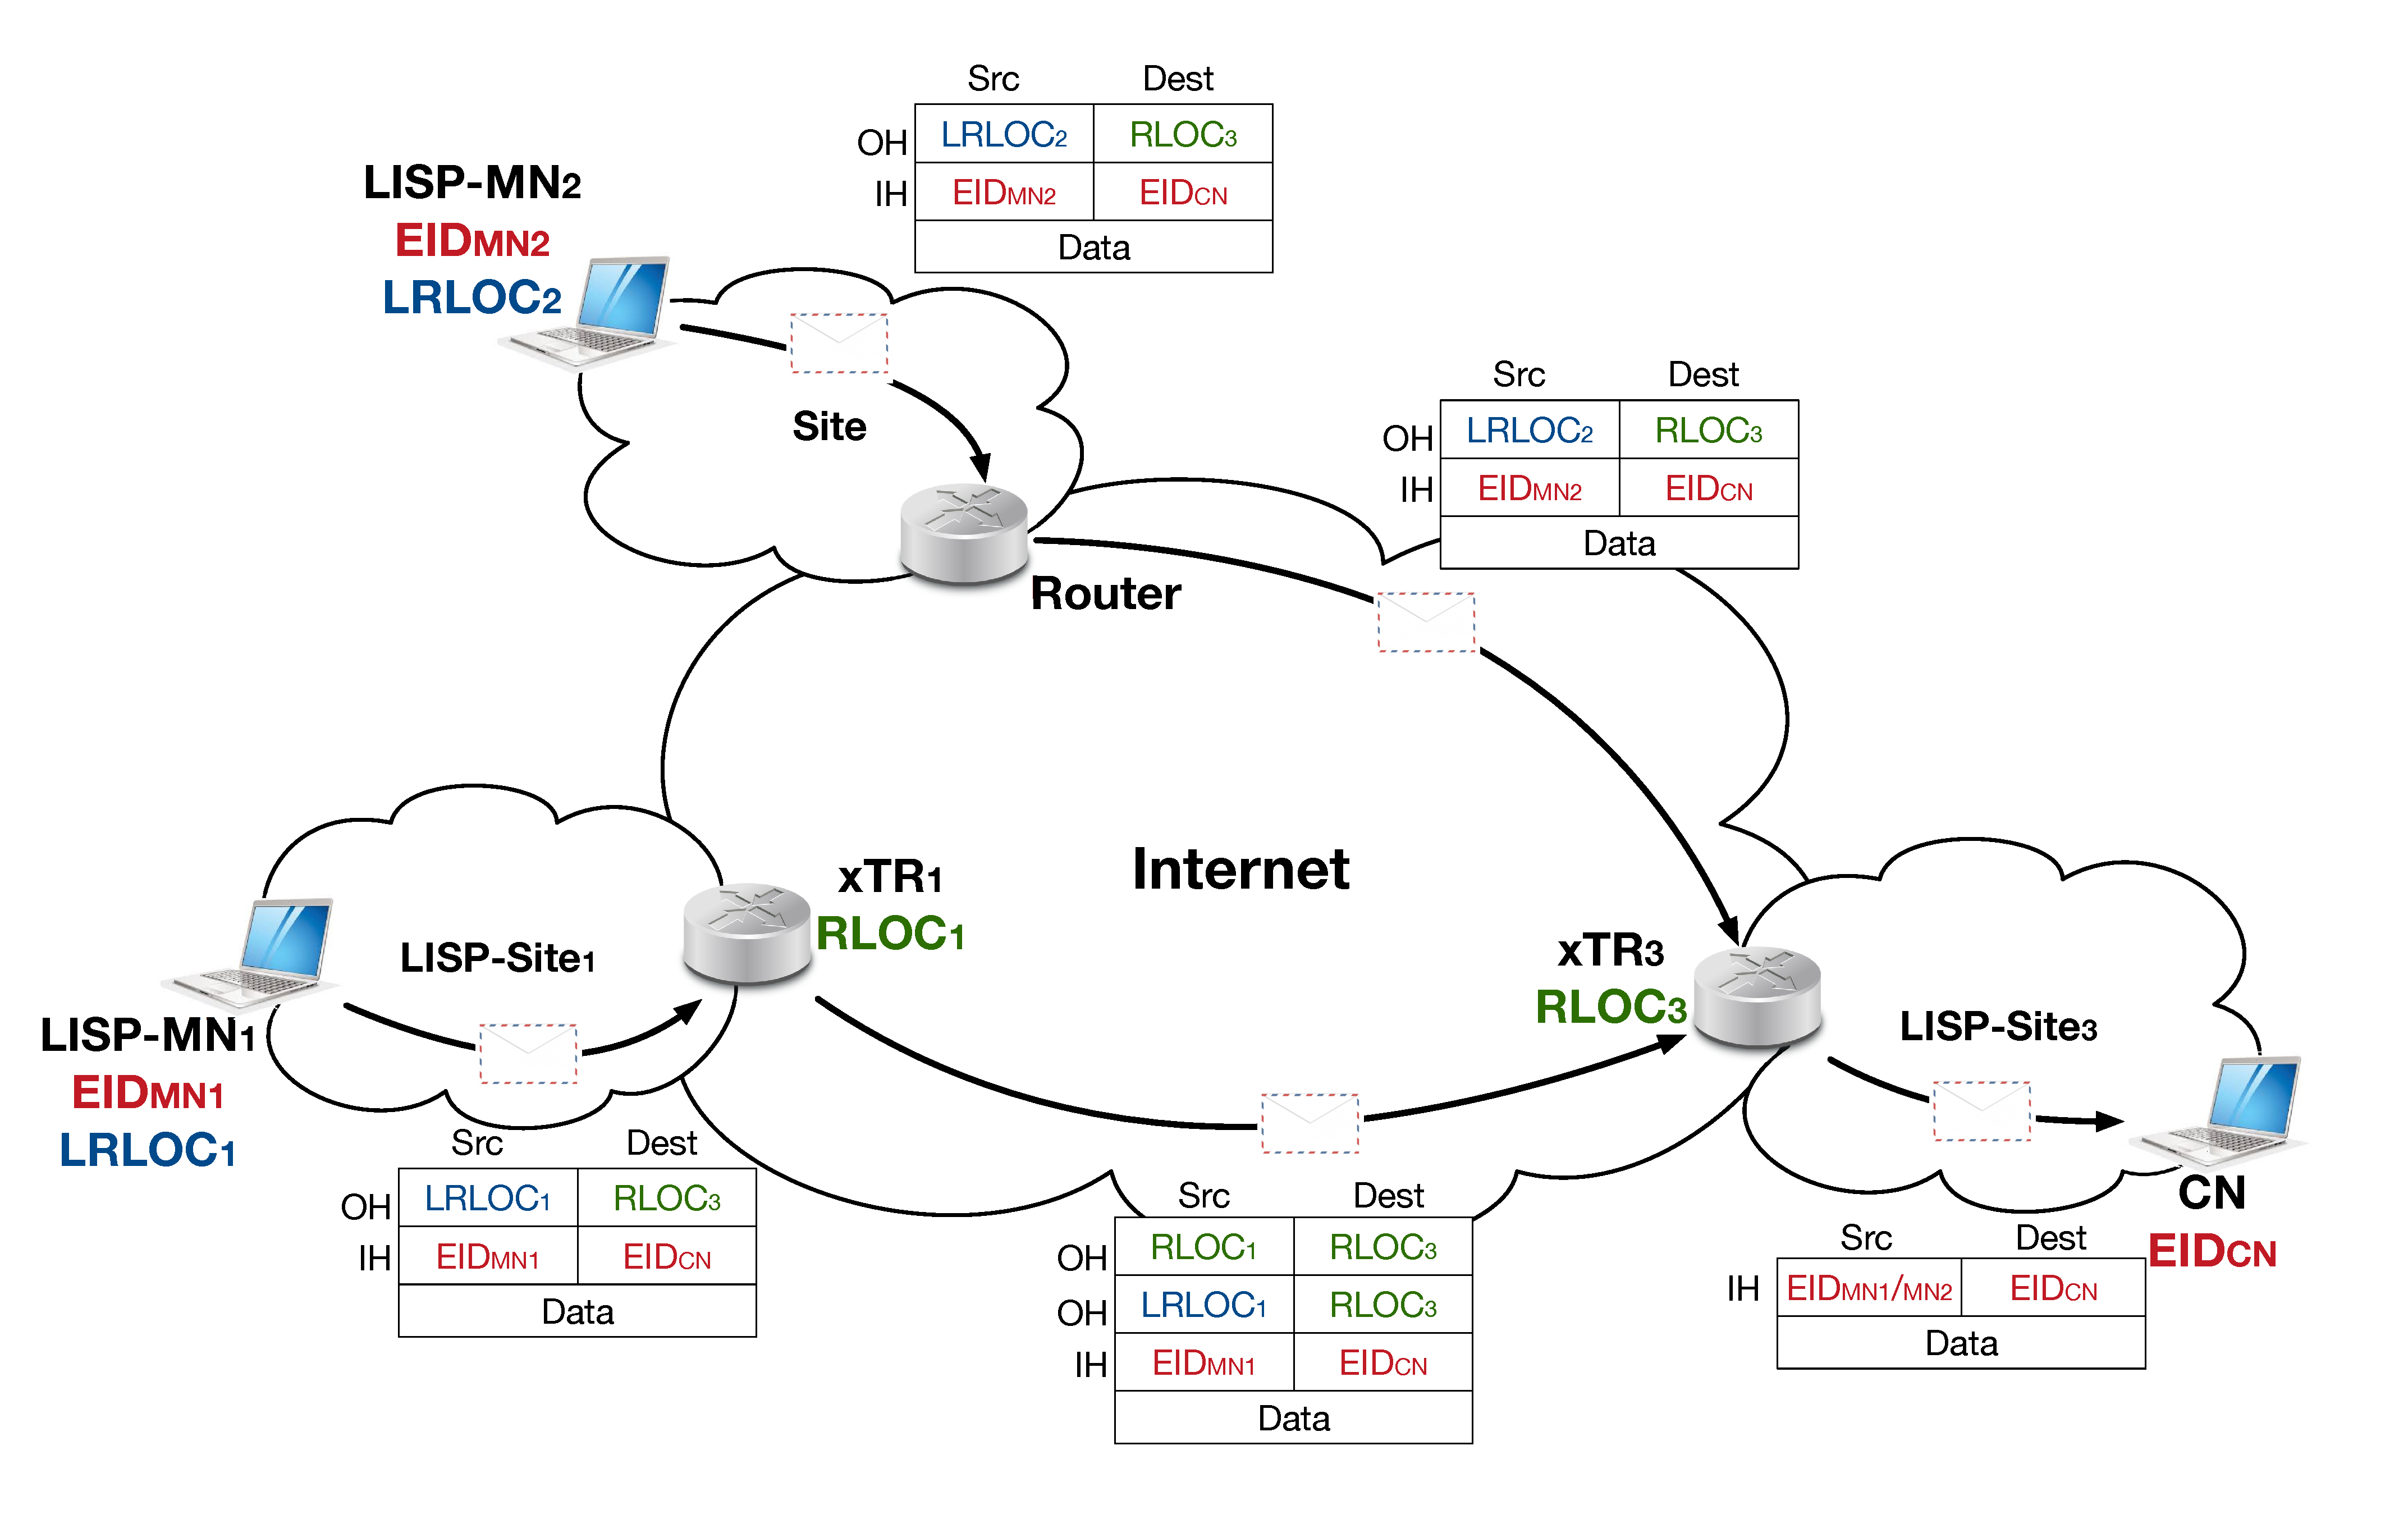
\includegraphics[width=\textwidth]{Pics/LISP-MN_archi.eps}
	\caption{Illustration of LISP-MN in LISP-Site and non-LISP-Site}
	\label{LISP_archi_2encap}
\end{figure}
%-< END FIGURE >--------------------------------------------------------------------
When a LISP-MN resides in a LISP-Site, it is assigned an EID taken from the site's EID-prefix as its RLOC, called \emph{\acrfull{lrloc}}. Thus, LISP-MN stores not only its permanent unique EID but also the \acrshort{lrloc} and registers this mapping information to the \acrshort{ms}. The conventional IP packets produced by the \acrshort{lispmn} are encapsulated by itself using the permanent EID as the inner source address and \acrshort{lrloc} as the outer source address. The encapsulated LISP packets are forwarded to \acrshort{xtr}s and encapsulated again. % by the method of basic LISP encapsulation. % The procedure of packets being encapsulated two times are called \emph{LISP double encapsulation}.

When a LISP-MN resides in a non-LISP-Site, it is assigned an IP address taken from the site's prefix as its \emph{\acrshort{lrloc}}. LISP-MN also need to store both its permanent unique EID and the \acrshort{lrloc} and register this mapping information to the \acrshort{ms}. The conventional IP packets produced by the \acrshort{lispmn} are encapsulated by itself using the permanent EID as the inner source address and \acrshort{lrloc} as the outer source address. The encapsulated LISP packets are forwarded to the border router and natively forwarded to the Internet core. 

The packet flow sequence of \acrshort{lispmn} in LISP-Site and non-LISP-Site are shown in Fig.~\ref{LISP_archi_2encap}. Two \acrshort{lispmn}s, i.e., $\text{LISP-MN}_1$ and $\text{LISP-MN}_2$ send the packets to a remote \acrfull{cn} . The only difference is that $\text{LISP-MN}_1$ resides in a LISP-Site, while $\text{LISP-MN}_2$ resides in a non-LISP-Site. The $\text{LISP-MN}_1$ produces the traditional IP packets with $EID_{MN1}$ as source address and $EID_{CN}$ as destination address. Then it encapsulates by adding $LRLOC_1$ as outer source address and $RLOC_3$ as outer destination address by itself after querying the mapping information. The LISP packets with one time encapsulation are forwarded to $xTR_1$. The latter gets the mapping information from \acrshort{mr} and encapsulates once again the packets by adding the $RLOC_1$ as the outer source address and $RLOC_3$ as the outer destination address, then sends the double LISP encapsulated packets on core Internet. The $xTR_3$ needs to dencapsulate the packets twice after receiving and verifying the packets, and finally sends to $CN$.

The situation for $\text{LISP-MN}_2$ is simpler. It also produces the traditional IP packets and encapsulates the packets by itself, then sends to its border router. The $Router$ does nothing related to LISP but only forwards the already LISP-encapsulated packets to the Internet core. Thus, the packets are encapsulated only once, whose inner source and destination address is respectively $EID_{MN2}$ and $EID_{CN}$, outer source and destination address is respectively $LRLOC_2$ and $RLOC_3$.


%-< SUBSECTION >--------------------------------------------------------------------
\subsection{MN mobility in LISP-Site}
\label{subsec:MN_LS}
When the \acrshort{mn} is normal host without any LISP function, while the border router supports LISP, i.e., \acrshort{xtr}, the packets are exchanged with the remote $CN$ as the basic communication between two LISP-Sites introduced in Sec.~\ref{sec:communication_2_lisp}. The \acrshort{eid} of \acrshort{mn} is distributed from the EID-prefix of the LISP-Site, if \acrshort{mn} moves to a new LISP-Site but keeps the original \acrshort{eid}, it can not exchange the packets with its new \acrshort{xtr}, since its \acrshort{eid} does not belong to the EID-prefix of the new LISP-Site. Thus, in this case, the mobility of \acrshort{mn} can only conduct within a subnet instead of roaming through different domains.


%-< SUBSECTION >--------------------------------------------------------------------
\subsection{LISP-MN mobility in LISP-Site}
\label{subsec:lispMN_LS}

%-< FIGURE >--------------------------------------------------------------------
\begin{figure}[!t]
	\centering
	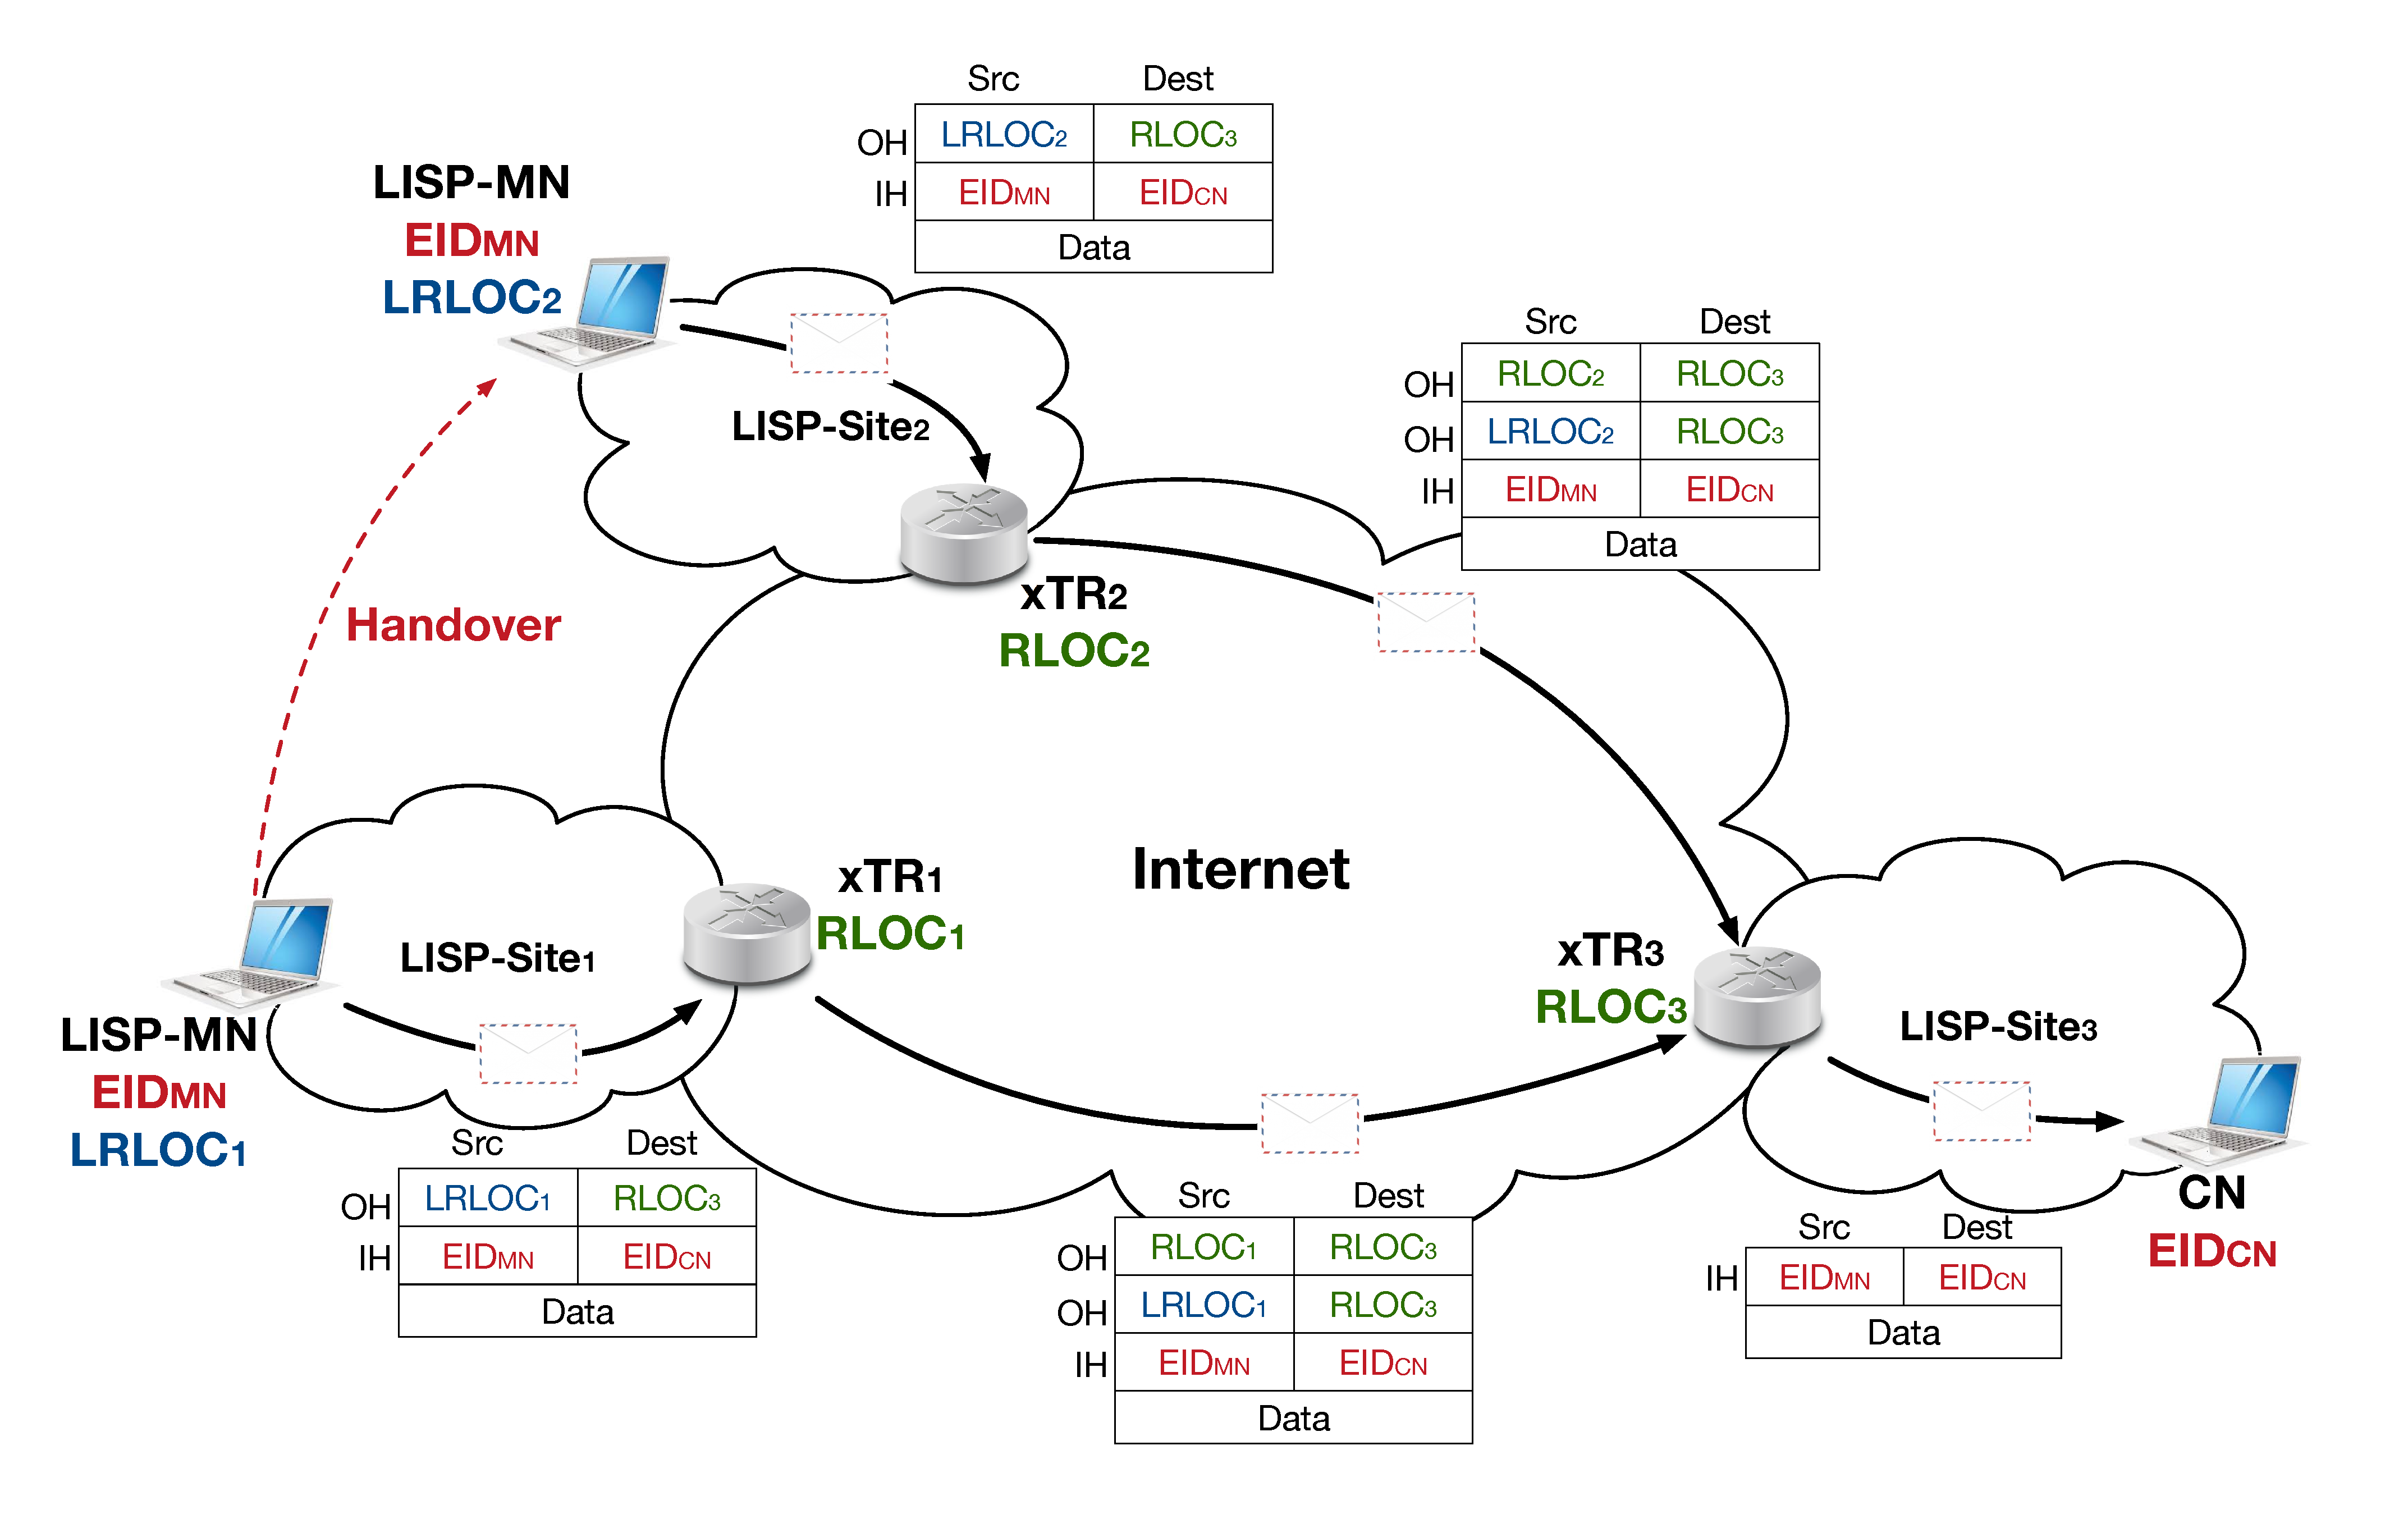
\includegraphics[width=\textwidth]{Pics/LISP-MN_in_LISP-Site.eps}
	\caption{Packet flow of mobility when LISP-MN in LISP-Site}
	\label{LISP-MN_in_LISP-Site}
\end{figure}
%-< END FIGURE >--------------------------------------------------------------------

This section describes how a \acrshort{lispmn} moves from one LISP-Site to another and the packet flow is shown in Fig.~\ref{LISP-MN_in_LISP-Site}. At first, packets exchanged between $\text{LISP-MN}$ residing in $\text{LISP-Site}_1$ and $CN$ are double encapsulated LISP packets as mentioned in Sec.~\ref{subsec:lispMN}. After conducting the handover, $\text{LISP-MN}$ still uses its permanent $EID_{MN}$. However, since it changes the attachment point, $xTR_2$ distributes a new EID from its EID-prefix to it, and it uses this as its new \acrshort{lrloc}, labeled $LRLOC_2$ in the figure. The $\text{LISP-MN}$ should register itself with the new mapping information to the \acrshort{mds} and ask $CN$ to update its LISP-Cache by \acrshort{smr} or Map-Versioning (introduced in Sec.~\ref{sec:updateMechanisms}). When receiving the packets from $\text{LISP-MN}$, the $xTR_2$ conducts the second encapsulation and sends the packets to $xTR_3$. The benefit of such mobility is that the $\text{LISP-MN}$ can roam through the different subnets without interrupting the communication with the remote $CN$, because $\text{LISP-MN}$ never changes its EID. However, to conduct double registration may lead to higher delay of handover.

%-< SUBSECTION >--------------------------------------------------------------------
\subsection{LISP-MN mobility in non-LISP-Site}
\label{subsec:lispMN_NLS}

%-< FIGURE >--------------------------------------------------------------------
\begin{figure}[!t]
	\centering
	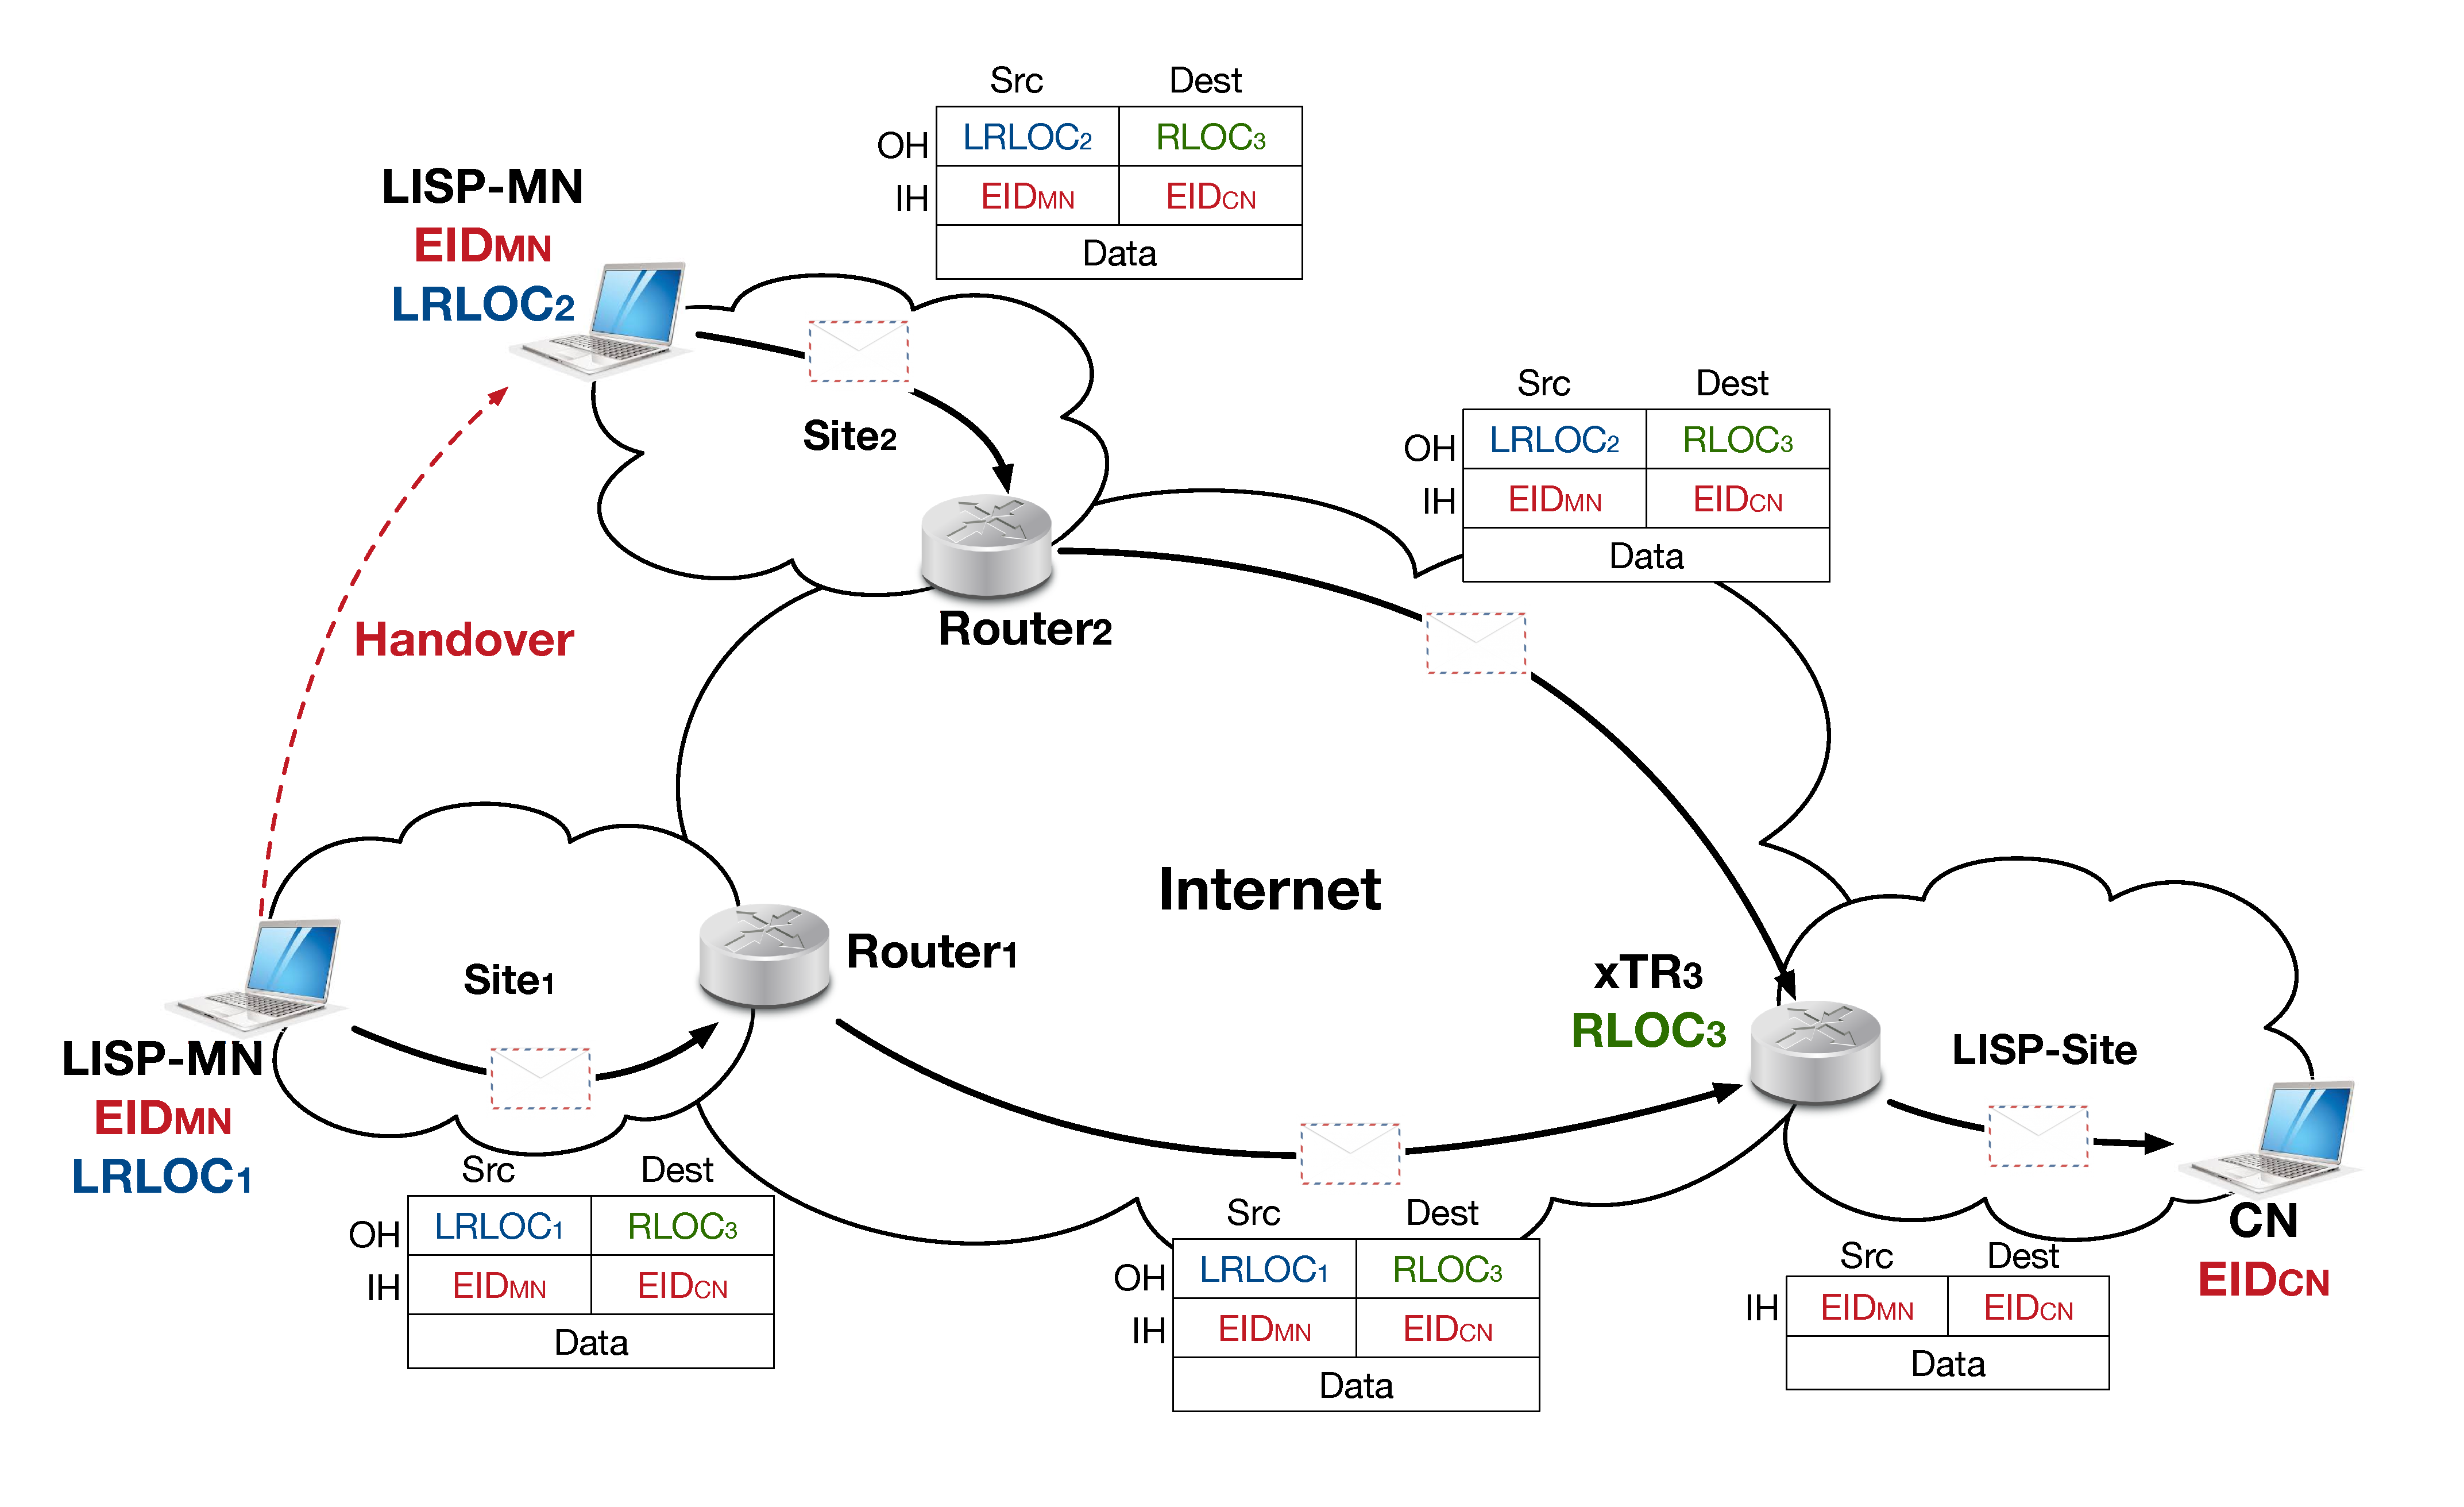
\includegraphics[width=\textwidth]{Pics/LISP-MN_in_non-LISP-Site.eps}
	\caption{Packet flow of mobility when LISP-MN in non-LISP-Site}
	\label{LISP-MN_in_non-LISP-Site}
\end{figure}
%-< END FIGURE >--------------------------------------------------------------------
The Fig.~\ref{LISP-MN_in_non-LISP-Site} illustrates the packet flow of the $\text{LISP-MN}$ roaming between two non-LISP-Sites. The $Site_1$ distributes an IP address from its prefix to $\text{LISP-MN}$, and the later uses this as its \acrshort{lrloc}, labeled as $LRLOC_1$ in the figure. The $\text{LISP-MN}$ encapsulates the packets by itself and sends to $Router_1$. $Router_1$ just natively forwards the packets to $xTR_3$. When $\text{LISP-MN}$ moves to another site labeled $Site_2$, it receives an IP address from a different prefix and uses it as the new \acrshort{lrloc}. It registers itself to the \acrshort{mds} with the $EID_{MN}\text{-to-}LRLOC_2$, and informs the remote $CN$ to update the mapping information by sending \acrshort{smr} or using Map-Versioning. In this scenario, $\text{LISP-MN}$ can also permit to roam through the different subnets, but it can also reduce the high latency of double registration during the handover. 


 %-< SUBSECTION >--------------------------------------------------------------------
 \subsection{LISP-MN mobility between LISP-Site \&  non-LISP-Site}
 \label{subsec:MN_NLS}

%-< SUB SECTION >--------------------------------------------------------------------
\section{LISP alternative use-cases}
\label{subsec:studies_usecase}
% State LISP use-cases
%     \begin{itemize}[noitemsep,topsep=0pt]
%         \item Traffic Engineering~\cite{rfc7834}
%         \item Transmission Between IPv4 and IPv6~\cite{rfc7834}
%         \item Mobility at User-side \yue{Cisco: Locator ID Separation Protocol (LISP) VM Mobility Solution, Support for Network-based User Mobility with LISP}
%         \item Mobility in Data Center \yue{Patrick's thesis + Cisco solution}
%         \item LISP SDN~\cite{barkai2017lisp}~\cite{han2016design}
%     \end{itemize}
Even though LISP is proposed to solve the Internet scalability issues, it also provides the advantages to the other uses, such as: traffic engineering, transition between IPv4 and IPv6, device's mobility at client-side, virtual machine's mobility in data center, LISP SDN, and so on~\cite{rfc7834}. 

%-< SUBSUB SECTION >--------------------------------------------------------------------
\subsection{LISP traffic engineering}
\label{subsubsec:te}
For every mapping information, an EID-prefix associates to a list of RLOC tuples $<$RLOC, Priority, Weight$>$, where each RLOC is annotated with a priority and a weight. In the case of multiple RLOCs existing, the ITR selects the one with the highest priority and sends all the LISP encapsulated packet to this RLOC. If several RLOCs all have the highest priority, the traffic is balanced proportionally according to their weight among such RLOCs so to route to multiple ETRs. Traffic engineering in LISP thus helps the mapping owner decide the primary and backup path for its incoming packets, and also allows it to control the traffic load among its links. For example, the received Map-Reply shows that an EID-prefix is associated to $<$RLOC\_1, 10, 50$>$, $<$RLOC\_2, 10, 20$>$, $<$RLOC\_3, 10, 20$>$, $<$RLOC\_4, 10, 10$>$, then the RLOC\_1 gets 50\% of the traffic, RLOC\_2 and RLOC\_3 are respectively assigned to 20\% of the traffic, and the last 10\% of the traffic are balanced by RLOC\_4.  % An example of the use of such a feature is described by Saucez et al. [SDIB08], which shows how to use LISP to direct different types of traffic on different links having different capacity.

Traffic engineering in LISP can achieve one step further than nowadays BPG. Since every Map-Request contains the source EID of the packet, for which causes the ITR mapping miss and triggers the Map-Request. It is possible that a mapping owner (ETR) gives the different Map-Replies according to the sender of Map-Requests. Thus, the traffic engineering policy may be different to different ITRs although they query the same ETR for the same EID-prefix. This functionality is not available today with BGP, because a domain cannot control exactly the incoming routes from the other domains if they are not direct neighbor.


%-< SUBSUB SECTION >--------------------------------------------------------------------
\subsection{LISP transition between IPv4 and IPv6}
\label{subsubsec:transmission}
The LISP encapsulation mechanism is designed to support any combination of address families for locators and identifiers, such as: IPv4, IPv6, MAC address, or some other arbitrary elements. It is then possible to bind IPv6 EIDs with IPv4 RLOCs and vice versa. This allows transporting IPv6 packets over an IPv4 network (or IPv4 packets over an IPv6 network) by deploying the xTRs at the border of heterogeneous networks, making LISP a valuable mechanism to ease the transition to IPv6.
%-< FIGURE >--------------------------------------------------------------------
\begin{figure}[!t]
	\centering
	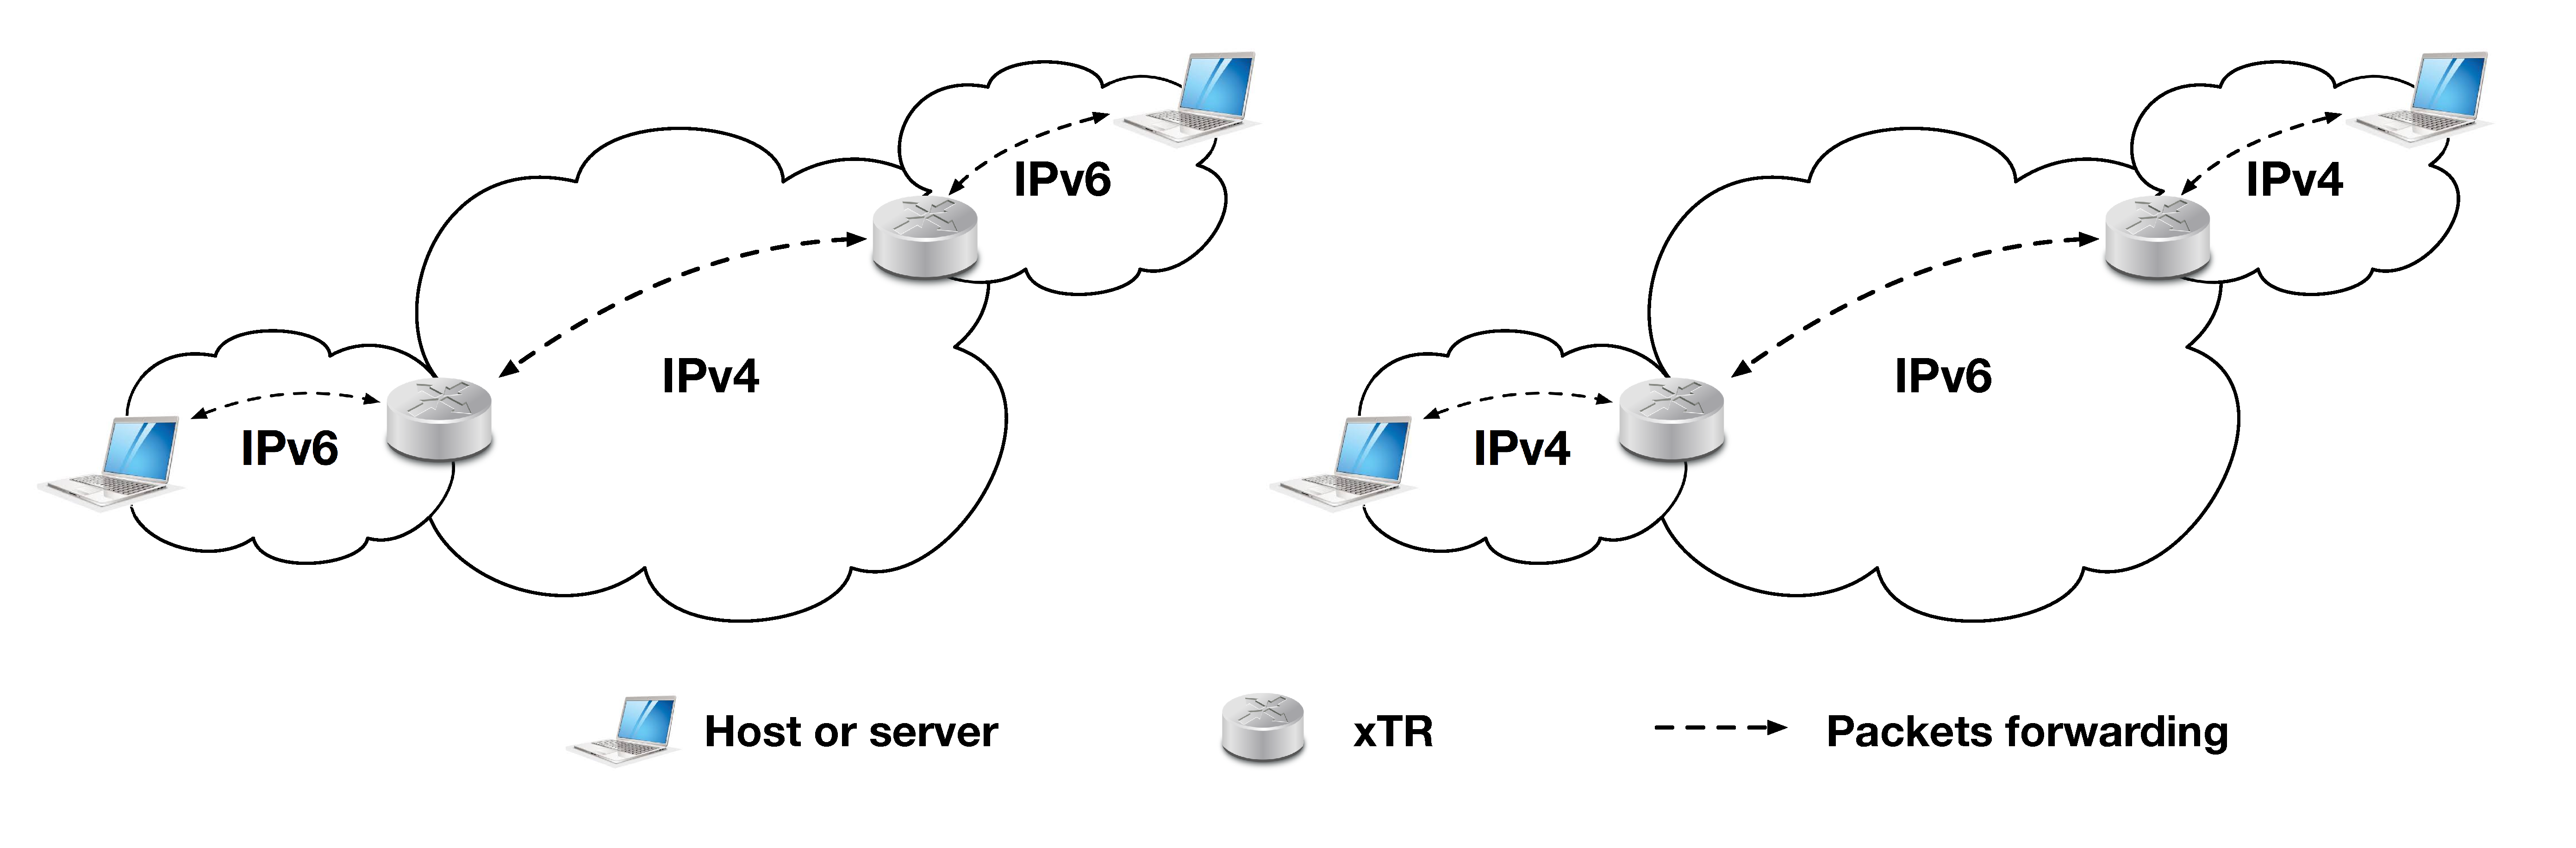
\includegraphics[width=\textwidth]{Pics/transmission_ipv4_ipv6.eps}
	\caption{Illustration of LISP transmission between IPv4 and IPv6}
	\label{transmission_ipv4_ipv6}
\end{figure}
%-< END FIGURE >--------------------------------------------------------------------

Examples are as shown in Fig.~\ref{transmission_ipv4_ipv6}, where IPv6 islands are connected via IPv4 infrastructure (on the left) and IPv4 islands are connected through IPv6 infrastructure (on the right). As LISP provides mechanisms for encapsulating IPv6 host packets using IPv4 RLOCs on the xTRs, LISP can then provide IPv6 communication between hosts/servers even though the intermediate network only supports IPv4. Similarly, xTR can encapsulate the IPv4 packets by adding the IPv6 RLOCs to achieve the IPv4 access through the IPv6 infrastructure. In addition, when the LISP infrastructure includes PxTRs, it can provide both IPv4 and IPv6 connectivity to non-LISP IPv4/IPv6 sites (legacy Internet). In summary, it can function in any of four following ways:
\begin{itemize}[noitemsep,topsep=0pt]
	\item IPv4-to-IPv4 over IPv4
	\item IPv4-to-IPv4 over IPv6
	\item IPv6-to-IPv6 over IPv4
	\item IPv6-to-IPv6 over IPv6
\end{itemize}
However, LISP does not translate between the IPv4 and IPv6 EIDs.



%%-< SUBSUB SECTION >--------------------------------------------------------------------
%\subsection{Mobility in Data Center}
%\label{subsubsec:mobility_DC}
%As the server virtualization and high availability across geographically dispersed data centers are more and more common, similar to the realization of LISP mobility at client-side, the migration of \acrfull{vm} within a data center or from a data center to another without dropping the running connections also becomes a potential use case of LISP. Two mechanisms at the state of the art can perform this operation. One is the aforementioned host-based LISP implementation called OOR, another method to handle \acrshort{vm} mobility via LISP is actually implemented in some Cisco products, only partially documented in~\cite{ciscovmmobility}. % The later one will be presented here.
%
%% The proposal of Cisco is based on the decoupling of Identifier from the topology so to ensure the changing of attachment point does not affect the EID. In the LISP VM-Mobility solution, only border routers of data center are embedded LISP, whereas VM is not, unlike \acrshort{lispmn}. When a VM moves to another subnet (i.e., it is paused, copied to another location, and then resumed), the VM restarts the DHCP procedure in order to obtain an suitable IP address for the new network. It does not continue to send traffic using the old IP, since it realizes that its attachment point has changed. As soon as the new xTR receives the DHCP, it realizes a VM moving from another subnet to its (i.e., it is paused, copied to another location, and then resumed) by detecting that the source IP of the traffic is not part of its EID-prefix (but it’s an allowed EID). The movement of VM is thus dynamically detected by xTR (the new LISP-VM router). After the new LISP-VM router detecting the newly moved-in VM, the new xTR needs to register the /32 for the VM's EID using its RLOC(s), and update the \acrshort{ms} by sending the Map-Register. Then, the MS replies 2 Map-Notifies: one is the acknowledge of Map-Register to the new xTR (the one who sent the Map-Register); the other one is to inform the previous xTR (which RLOCs were previously mapped to the VM's EID) to remove the mapping information for the leaving VM. Then, the previous xTR notifies the departure of VM by sending SMRs to every CN, which was communicating with the moved VM before. By updating the RLOC-to-EID mappings, traffic is redirected to the new locations without causing any churn in the underlying routing. As the VM is not aware of the move during the whole roaming, the LISP VM-Mobility solution is network-based mobility.


%-< SUBSUB SECTION >--------------------------------------------------------------------
\subsection{LISP SDN}
\label{subsubsec:sdn}
As described before, LISP is inherently decoupling Control Plane from Data Plane. LISP moves all control functions onto Mapping System, while keeps data functions at the xTR level.%\yue{Personally, I'm not agreed with this statement. Your writing makes me feel that xTR only supports data plane function. Actually it also support control plane functions...}
The feature of LISP corresponds to the characteristic of \acrfull{sdn}, which also decouples Network Control Plane from Data Plane, increases flexibility and development speed of features and functionalists. Thus, this decoupling entitles network operators to build a \acrfull{sdn} on top of LISP~\cite{rodriguez2014software}.

%-< FIGURE >--------------------------------------------------------------------
\begin{figure}[!t]
	\centering
	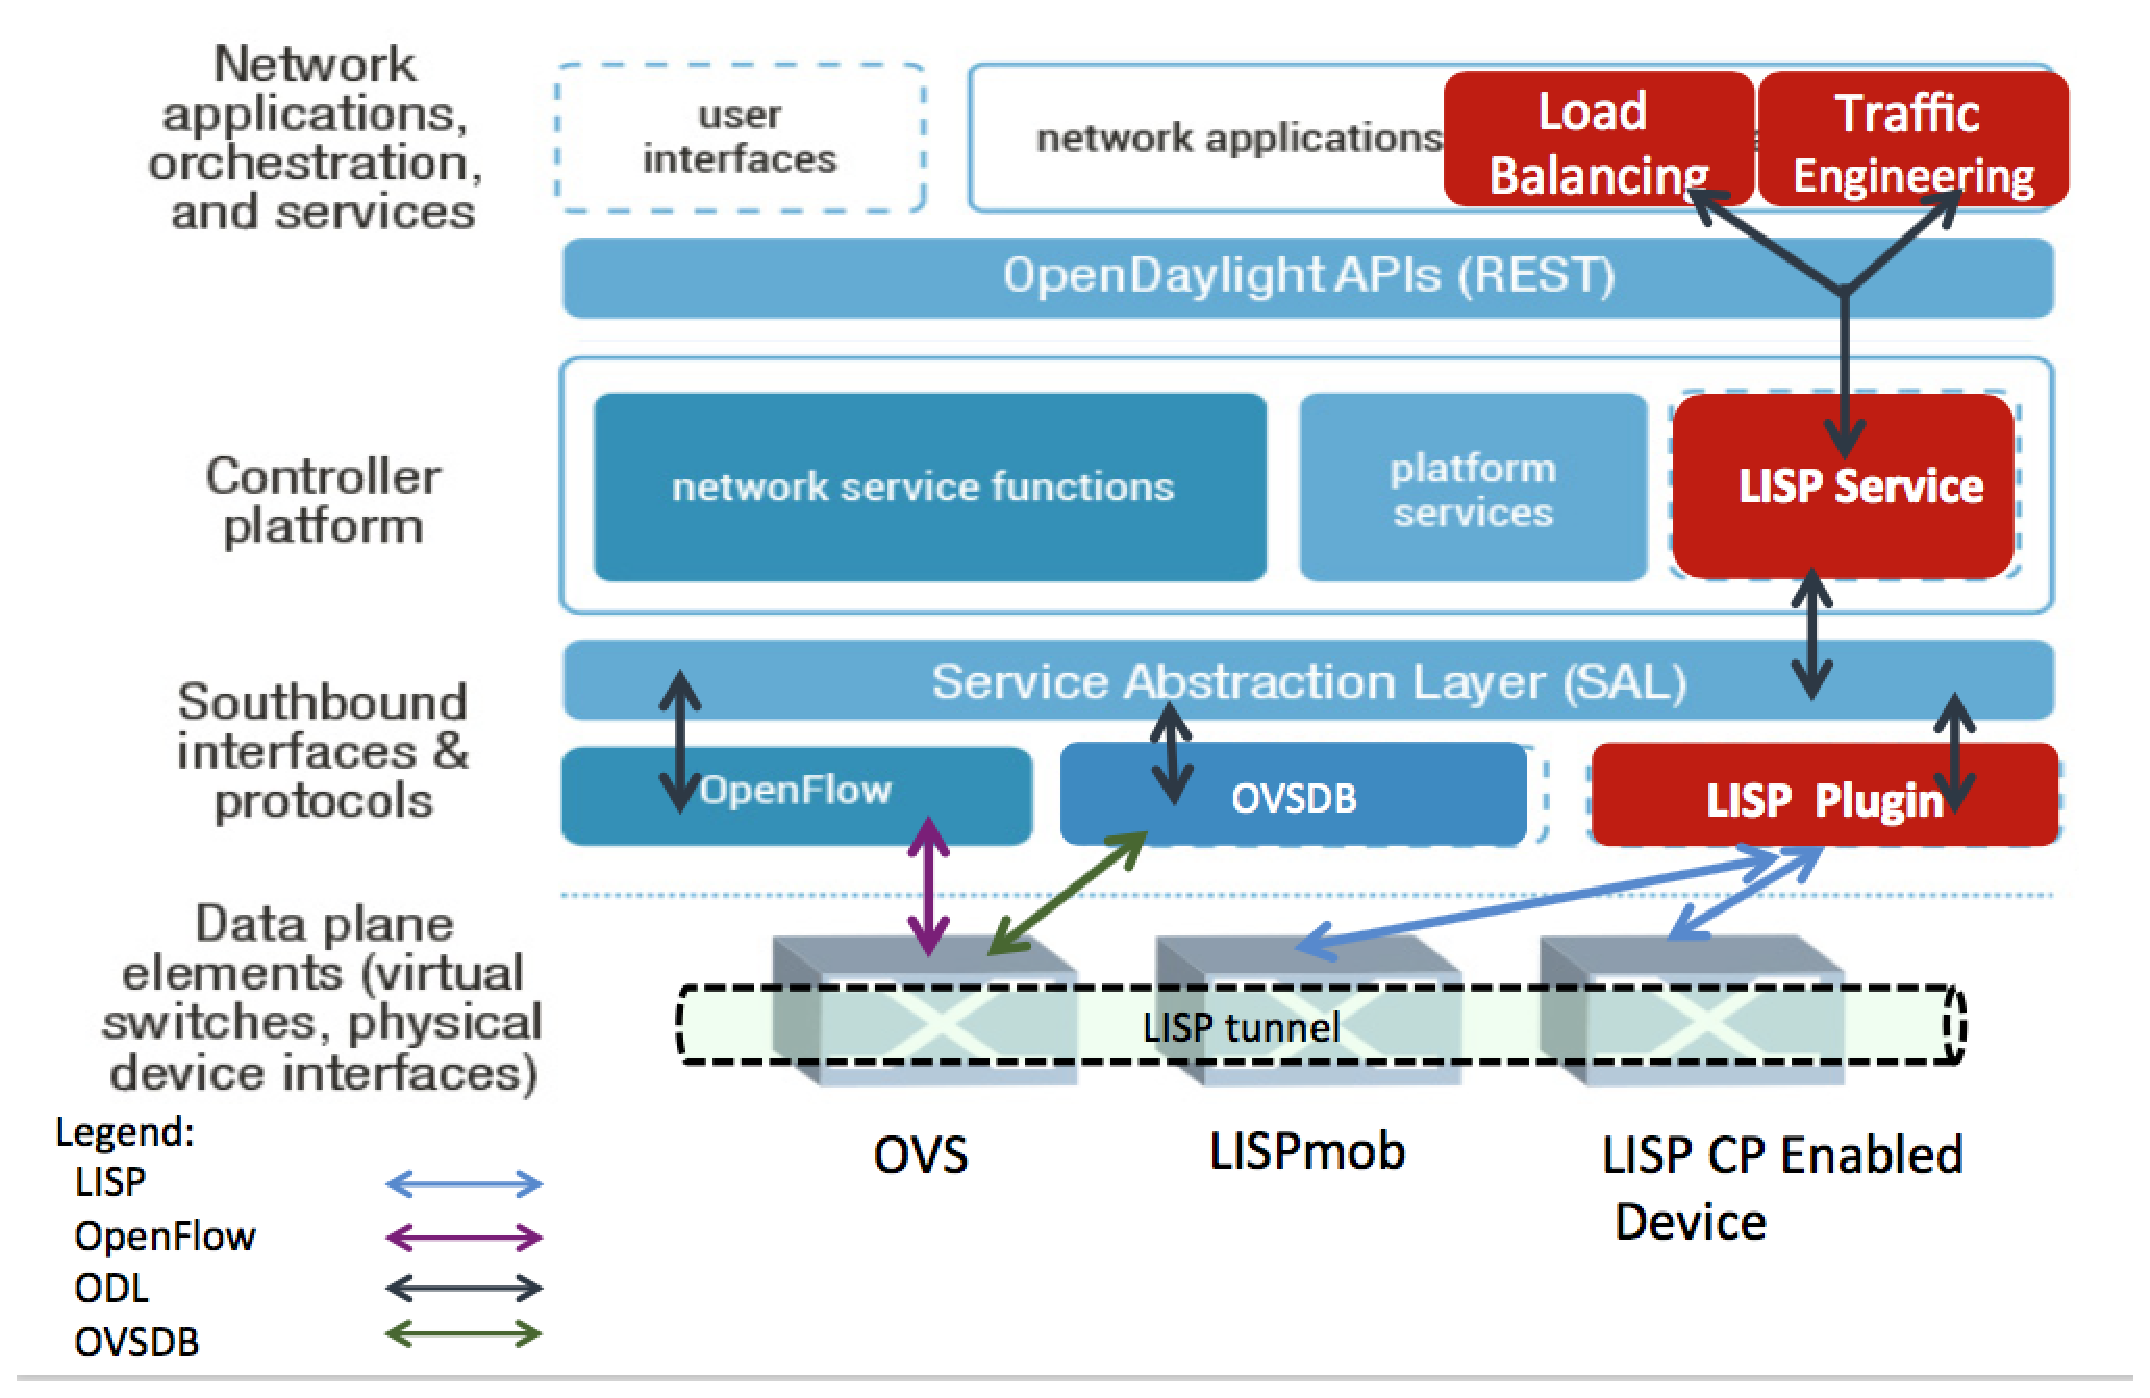
\includegraphics[width=\textwidth]{Pics/LISP_in_OpenDaylight.eps}
	\caption{LISP in OpenDaylight (source:~\cite{LISP_ODLSummit_2014})}
	\label{LISP_in_OpenDaylight}
\end{figure}
%-< END FIGURE >--------------------------------------------------------------------
The OpenDaylight Project~\cite{OpenDaylight} is a collaborative open source project hosted by The Linux Foundation to promote \acrfull{sdn} and \acrfull{nfv}. It implements the LISP Control Plane functions as shown in Fig~\ref{LISP_in_OpenDaylight}. The data plane elements consist of virtual switches and physical device interfaces, at the aim of constructing the LISP tunnel to transfer the packets. The LISP Plugin is the Southbound interface, which is used to look up LISP policies from LISP Service by sending Map-Request and receiving Map-Reply, and create the LISP tunnel over LISP overlay across the different kinds of data plane devices. The LISP Service is actually implemented as LISP Mapping System to store the various user-defined policies. The only difference is that in OpenDaylight, it is the \acrshort{ms} itself that replies to the Map-Requests, instead of forwarding them to any xTR. It is like every mapping has the "proxy Map-Reply" flag (P-bit) set to response on behalf of xTRs. The OpenDaylight APIs (REST) are used to set the policies, such as: the policies for Load Balancing and Traffic Engineering, obtained from the north bound into LISP Service. The policies are defined as the network applications or services by the users.

Network functions such as subscriber-management, content-optimization, security and quality of service, are typically delivered using proprietary hardware appliances embedded into the network~\cite{barkai2017lisp}. But the next generation network functions are being implemented as pure software instances running on standard servers. They are unbundled virtualized components of capacity and functionality. LISP-SDN based flow-mapping, dynamically assembles these components to whole solutions by steering the proper traffic in the right sequence to the correct virtual function instance.
